\documentclass[a4paper,12pt,openany]{book}
% ------------------------------------------------------------------------
% pakiet do wzorów ams
% ------------------------------------------------------------------------
\usepackage{amsmath}
\usepackage{amssymb}

% ------------------------------------------------------------------------
% język polski
% ------------------------------------------------------------------------
\usepackage[MeX]{polski}
%\usepackage[cp1250]{inputenc}

\usepackage[utf8x]{inputenc}

% ------------------------------------------------------------------------
% obsługa pdf
% ------------------------------------------------------------------------
\usepackage[pdftex,usenames,dvipsnames]{color}	%obsługa kolorów

% ------------------------------------------------------------------------
% wstawienie danych o autorze i pracy 
% ------------------------------------------------------------------------
\usepackage[pdftex,
				pagebackref=false,						% referencje w spisie literatury do strony na, której została urzyta
				draft=false,								% draft
				pdfpagelabels=false,						%
				pdfstartview=FitV,						% lub FitH
				pdfstartpage=1,							% 
				bookmarks=true,							% zakładki w pliku pdf
				pdfauthor={Autor},						% należy wpisać autora pracy
				pdftitle={Praca inżynierska},			% 
				pdfsubject={Tytuł pracy},				% tytuł
				pdfkeywords={slowa kluczowe},			% slowa kluczowe
				unicode=true]{hyperref}   


% ------------------------------------------------------------------------
%	style
% ------------------------------------------------------------------------
\usepackage{extsizes}							%wiecej rozmiarów czcionek
\usepackage[a4paper,left=3.5cm,right=2.5cm,top=2.5cm,bottom=2.5cm]{geometry}
\usepackage{tocloft}								% format spisu treści
\usepackage{array}								% lepiej wyglądające tabelki
\usepackage[format=hang,
				labelsep=period,
				labelfont={bf,small},
				textfont=small]{caption}		% formatuje podpisy pod rysunkami i tabelami
\usepackage{floatflt}							% ładniejsze opisywanie obrazków tekstem
\usepackage{subfig}								% możliwość wstawiania figur w kolumnach
\usepackage{graphicx}							% do obsługi grafiki
\usepackage{here}									% wymuszanie położenia figury w danym miejscu
\usepackage{url}									% adresy internetowe
\usepackage{enumerate}							% modyfikowanie list wyliczeniowych np \begin{enumerate}[(a)]...
\usepackage{multirow}							% do tabel 
% ------------------------------------------------------------------------
% listingi
% ------------------------------------------------------------------------
\usepackage{listings}							% do wstawiania listingow programów




\usepackage{slantsc} % Pochyłe kapitaliki  np. \textsl{\textsc{Automatyka i robotyka}}

% ------------------------------------------------------------------------
% inne
% ------------------------------------------------------------------------
\usepackage{glossaries}

\usepackage{dashrule}
\usepackage{fancyhdr} 							% do stopki i nagłówka
\usepackage{calc}
\usepackage{packages/zmienne}					% zmienne dodatkowe używane min. w karcie pracy oświadczeniu i stronie tytułowej zebrane w jednym miejscu
\usepackage{packages/strona_tytulowa}
\usepackage{packages/pusta_strona}
\usepackage{longtable}							% do podziału tabel na wiele stron

\usepackage{indentfirst}

% ------------------------------------------------------------------------
% kodowanie czcionek
% ------------------------------------------------------------------------
\usepackage[T1]{fontenc}
\usepackage{lmodern}\normalfont %to load T1lmr.fd 

% ------------------------------------------------------------------------
% do algorytmów
% ------------------------------------------------------------------------

\usepackage{algorithm}
\usepackage{algorithmic}
\floatname{algorithm}{Algorytm}

% ------------------------------------------------------------------------
% do nonmeklatury
% ------------------------------------------------------------------------

\usepackage[section]{placeins}
\usepackage{nomencl}
\makenomenclature
\usepackage{makeidx}
\makeindex
\renewcommand{\nomname}{Spis ważniejszych symboli}
% \newcommand{\pauza}{--}
% na końcu pliku z nomekaturą należy umieścić polecenie
% \printnomenclature
% plik należy dodać poleceniem \input
%% przykład treści pliku
%% \nomenclature{$\oplus$}{Dylatacja zbioru}
%% \printnomenclature





% ------------------------------------------------------------------------
%   Kropki po numerach sekcji, podsekcji, itd.
%   Np. 1.2. Tytuł podrozdziału
% ------------------------------------------------------------------------
\makeatletter
    \def\numberline#1{\hb@xt@\@tempdima{#1.\hfil}}                      %kropki w spisie treści
    \renewcommand*\@seccntformat[1]{\csname the#1\endcsname.\enspace}   %kropki w treści dokumentu
\makeatother

\makeatother
% ------------------------------------------------------------------------
% Definicje
% ------------------------------------------------------------------------
\def\nonumsection#1{%
    \section*{#1}%
    \addcontentsline{toc}{section}{#1}%
    }
\def\nonumsubsection#1{%
    \subsection*{#1}%
    \addcontentsline{toc}{subsection}{#1}%
    }
\reversemarginpar %umieszcza notki po lewej stronie, czyli tam gdzie jest więcej miejsca
\def\notka#1{%
    \marginpar{\footnotesize{#1}}%
    }
%\def\mathcal#1{%
%    \mathscr{#1}%
%    }

\newcommand{\myemptypage}{ \newpage  \thispagestyle{empty}~\newpage}

%-------------------------------------------------------------------------
% listingi
%-------------------------------------------------------------------------
\lstdefinestyle{praca}{basicstyle=\scriptsize\ttfamily, 
								keywordstyle=\color{black}\bfseries,
								numbers=left, 
								stepnumber=1, 
								numberstyle=\tiny, 
								numbersep=10pt,
								extendedchars=true, 
								frame=tb}
\lstset{style=praca}

%-------------------------------------------------------------------------
% stopka i nagłówek
%-------------------------------------------------------------------------
\setlength{\headheight}{15pt}

\pagestyle{fancy}
\renewcommand{\chaptermark}[1]{\markboth{#1}{}}
\renewcommand{\sectionmark}[1]{\markright{#1}{}}

\fancyhf{}
\fancyhead[LE,RO]{\thepage}
\fancyhead[RE]{\textit{\nouppercase{\leftmark}}}
\fancyhead[LO]{\textit{\nouppercase{\rightmark}}}

\fancypagestyle{plain}{ %
\fancyhf{}
\renewcommand{\headrulewidth}{0pt}
\renewcommand{\footrulewidth}{0pt}}

% ------------------------------------------------------------------------
% Inne
% ------------------------------------------------------------------------
\frenchspacing
\setlength{\parskip}{3pt}           	%odstęp pomiędzy akapitami
%\linespread{1.49}                    	%odstęp pomiędzy liniami (interlinia)
\setcounter{tocdepth}{3}
\setcounter{secnumdepth}{3}


% ------------------------------------------------------------------------
% Polskie podpisy
% ------------------------------------------------------------------------
\renewcommand{\figurename}{Rys.}
\renewcommand{\tablename}{Tab.}

% ------------------------------------------------------------------------
% Bibliografia
% ------------------------------------------------------------------------
\bibliographystyle{unsrt}					% kolejność według użycia
%\bibliographystyle{plain}					% kolejność alfabetyczna
  
  

%==========================================================================================
% Deklaracja fontów kapitalikowych z kodowaniem T1
%==========================================================================================
\DeclareFontShape{T1}{lmr}{bx}{sc} { <-> ssub * cmr/bx/sc }{}
\DeclareFontShape{T1}{lmr}{bx}{scit}{<-> ssub * cmr/bx/scsl}{}
%==========================================================================================
% Inne deklaracje
%==========================================================================================


\usepackage{xcolor}

\definecolor{codegreen}{rgb}{0,0.6,0}
\definecolor{codegray}{rgb}{0.5,0.5,0.5}
\definecolor{codepurple}{rgb}{0.58,0,0.82}

\lstdefinestyle{mystyle}{   
    commentstyle=\color{codegreen},
    keywordstyle=\color{magenta},
    numberstyle=\tiny\color{codegray},
    stringstyle=\color{codepurple},
    basicstyle=\ttfamily\footnotesize,
    breakatwhitespace=false,         
    breaklines=true,                 
    captionpos=b,                    
    keepspaces=true,                 
    numbers=left,                    
    numbersep=5pt,                  
    showspaces=false,                
    showstringspaces=false,
    showtabs=false,                  
    tabsize=2
}
\lstset{style=mystyle}

\definecolor{lightgray}{rgb}{.9,.9,.9}
\definecolor{darkgray}{rgb}{.4,.4,.4}
\definecolor{purple}{rgb}{0.65, 0.12, 0.82}

\lstdefinelanguage{JavaScript}{
  keywords={typeof, new, true, false, catch, function, return, null, catch, switch, var, if, in, while, do, else, case, break},
  keywordstyle=\color{blue}\bfseries,
  ndkeywords={class, export, boolean, throw, implements, import, this},
  ndkeywordstyle=\color{darkgray}\bfseries,
  identifierstyle=\color{black},
  sensitive=false,
  comment=[l]{//},
  morecomment=[s]{/*}{*/},
  commentstyle=\color{purple}\ttfamily,
  stringstyle=\color{red}\ttfamily,
  morestring=[b]',
  morestring=[b]"
}

\lstset{
   language=JavaScript,
   extendedchars=true,
   basicstyle=\footnotesize\ttfamily,
   showstringspaces=false,
   showspaces=false,
   numbers=left,
   numberstyle=\footnotesize,
   numbersep=5pt,
   tabsize=2,
   breaklines=true,
   showtabs=false,
   captionpos=b
}

\AtBeginDocument{%
\renewcommand\lstlistlistingname{Spis fragmentów kodu}
}

%==========================================================================================

%==========================================================================================
% Dane na temat pracy do wypełnienia
%==========================================================================================
\author{Krystian Skibiński}
\kierunek{Informatyka}
\grupa{}
\title{Mikrousługi i Rozwiązania Monolityczne w Aplikacjach Internetowych}
\tytulAngielski{Microservices and Monolithic Solutions in Web Applications}
\uczelnia{}
\wydzial{}
\praca{Praca magisterska}
\promotor{}
\konsultant{} 	% nie usuwać w~przypadku braku lecz pozostawić puste czyli: \konsultant{}
%\konsultant{}
\miasto{Zielona Góra}
\miesiac{czerwiec}	% miesiąc złożenia pracy
\rok{2020}
\dzien{30} 			% dzień podpisania oœwiadczenia (cyfrowo) np. 10
\mm{06} 				% miesiac podpisania oœwiadczenia (cyfrowo) np. 01 (styczeń)

%==========================================================================================
% Dokument głowny
%==========================================================================================
\begin{document}
\pagenumbering{roman}
%=========================================================================================
% Strona tytułowa
%=========================================================================================
\thispagestyle{empty}

\stronatytulowa

\thispagestyle{empty}
\pustastrona
\newpage

%========================================================================================
% Streszczenie
%========================================================================================
\normalsize

\subsection*{Streszczenie}

Praca dotyczy porównania dwóch popularnych podejść, mikrousługowego~i monolitycznego, stosowanych przy tworzeniu serwisów internetowych. Jej celem jest przedstawienie podobieństw~i różnic między tymi wzorcami, a także ich właściwości~i wskazanie przypadków, dla których najlepiej sprawują się dane architektury. Na jej potrzeby stworzono dwa serwisy internetowe~z wykorzystaniem omawianych podejść. Następnie przedstawiono konfigurację ich środowisk~i potrzebnych narzędzi. Badania wykonane~w ramach pracy obejmowały sprawdzenie aplikacji pod kątem wydajności wysyłanych przez serwer żądań, a także skalowalności poziomej~i pionowej. Przeprowadzono również analizę implementacji aplikacji~i zastosowanych technologii. W rezultacie pozwoliło to na wskazanie wad~i zalet obu podejść, ocenie, kiedy najlepiej zastosować jedną~z nich~i zaproponowaniu możliwych ulepszeń~w architekturze projektu.

\vspace{1cm}
\noindent\textbf{Słowa kluczowe:} praca dyplomowa, aplikacje internetowe, mikrousługi, monolit, architektura serwisów internetowych.

\newpage
%\myemptypage

%========================================================================================
% Spis treści, spis tabel i~rysunków
%========================================================================================
%spis treści
	\tableofcontents
	\newpage
	%\myemptypage
%spis rysunków
 	\listoffigures
	\newpage
	%\myemptypage
%spis tabel
	\listoftables
	\newpage
	%\myemptypage
%spis listingów
	\lstlistoflistings
	\newpage

%========================================================================================
% Licznik Stron
%========================================================================================
\newcounter{licznikStron}
\setcounter{licznikStron}{\value{page}}
\setcounter{licznikStron}{1}
\pagenumbering{arabic}
\setcounter{page}{\value{licznikStron}}

%========================================================================================
% Treść
%========================================================================================
\chapter{Wstęp}
%======================================================================================================
Celem niniejszej pracy było zaprojektowanie aplikacji pod kątem architektury opartej~o podejście monolityczne~i mikrousługi. W jej ramach przygotowano dwa serwisy, a następnie starannie opisano proces ich implementacji~i konfigurację. Szczególnie ważne było to, aby oba serwisy były napisane~w ramach tych samych technologii~i narzędzi, tak żeby można je było odpowiednio porównać. Szczegółowo przedstawiono również proces konteneryzacji projektu, tak aby, mógł on zostać~w łatwy sposób zintegrowany~z platformą dostarczającą rozwiązania internetowe.

W ramach porównania obu serwisów przeprowadzono testy wydajnościowe, sprawdzono możliwości skalowania aplikacji~i wpływ tej technologii na ich sprawność, a następnie poddano analizie dostarczone rozwiązania architektoniczne, łatwość wdrożenia~i wykorzystane technologię. Dzięki temu możliwe było opracowanie wniosków, których celem było wskazanie wad~i zalet, a także przypadków dla których najlepiej sprawuje się dana architektura.

Tekst pracy oparto głownie~o pozycję \cite{Ziade:2018}, gdzie autor również przygotował aplikację opartą~o mikrousługi, opisał jej architekturę~i przedstawił narzędzia potrzebne do jej implementacji, ale także inne pozycje takie jak \cite{Rodger:2019}, czy \cite{Folwer:2019}, traktujące~o ideach stojących za oboma podejściami, ich charakterystykami, wadami~i zaletami. We wszystkich książkach znajdowały się cenne rozdział poświęcone analizie przypadków, czy pomysłami na wdrożenie konkretnej architektury.

Przygotowana praca powinna pomóc~w wybraniu odpowiedniej architektury, przedstawiono~w niej proces przygotowania serwisu internetowego wraz~z analizą załączonego kodu. Czytelnik po jej przeczytaniu powinien móc odtworzyć prostą aplikację opartą~o oba podejścia, przygotować ich strukturę~i integrację~z środowiskiem produkcyjnym przy pomocy narzędzia do konteneryzacji. Następnie analizując badania~i ich wyniki, a także wnioski autora, móc wybrać najlepszą~z architektur dla jego własnego zastosowania.

Praca składa się~z rozdziału \ref{roz2}., gdzie omówiono główne założenia aplikacji internetowych, a następnie wyjaśniono strukturę architektury monolitycznej~i podejścia opartego~o mikrousługi. Przedstawione zostało studium przypadku serwisu internetowego, gdzie wdrożony byłby model scentralizowany~i rozwiązanie oparte~o mniejsze usługi.

W rozdziale \ref{roz3}. omówiono projekt dwóch serwisów internetowych, opisano jego założenia, możliwe problemy które mogą zaistnieć~w trakcie jego implementacji~i dostępne rozwiązania. Następnie uszczegółowiono architektury poszczególnych aplikacji. Wyjaśniono relację, które wykorzystane będą~w bazie danych, a także potrzebne biblioteki. Przeprowadzono również analizę wymagań funkcyjnych~i niefunkcyjnych, a także opisano środowisko programistyczne, które będzie potrzebne do uruchomienia projektu~i wspierane przeglądarki.

Natomiast rozdziały \ref{roz4}. i \ref{roz5}. skupiają się na szczegółowym opisie implementacji danej architektury, są one podzielone według poszczególnych warstw biznesowych aplikacji.

Problem integracji~z platformami dostarczającymi rozwiązania~w zakresie hostingu aplikacji opisano~w rozdziale \ref{roz6}. Przedstawiono~w nim proces konteneryzacji aplikacji, a także przygotowania jej środowiska deweloperskiego~i produkcyjnego, tak, aby można było~w łatwy sposób ją rozwijać, a także dostarczyć użytkownikom.

W rozdziale \ref{roz7}. na środowisku produkcyjnym przeprowadzono  badania mające na celu sprawdzenie wydajności obu architektur. Przeanalizowano możliwości ich skalowania. Wpływ tego rozwiązania na sprawność systemu, a następnie analizie poddano cały projekt, tak, aby podsumować, która~z architektur jest łatwiejsza do implementacji.

W ostatnim rozdziale \ref{roz8}. przedstawiono wnioski po implementacji~i przetestowaniu obu aplikacji, następnie wskazano charakterystyki obu architektur, ich wady~i zalety. Przedyskutowano osiągnięte rezultaty, a na końcu wskazano, dla jakiego przypadku najlepszym rozwiązaniem jest dane podejście.
\chapter{Rodzaje aplikacji internetowych}
\label{roz2}
%=================================================================================================
\section{Aplikacje internetowe}
Szybko rosnąca popularność internetu~w latach 90. XX wieku sprawiła, że poza prostymi stronami \textit{HTML}\footnote{HTML(ang. \textit{HyperText Markup Language}), hipertekstowy język znaczników powszechnie używany do tworzenia stron internetowych. Źródło \url{https://www.w3.org/TR/html4/}} zaczęto budować bardziej skomplikowane portale internetowe, a następnie ogromne serwisy. Potrzeba większych~i lepszych systemów sprawiła,~że ich twórcy musieli znajdować coraz to nowsze sposoby na ich budowanie\cite{Newman:2016}. Obecnie popularnością\footnote{Według portalu \textit{Google Trends}, fraza ta zaczęła zdobywać popularność od około 2009 roku. Źródło \url{https://trends.google.com/trends/explore?date=all\&q=web\%20app,android\%20app,ios\%20app}} cieszą się aplikacje internetowe. Są to programy komputerowe, które wykorzystują przeglądarkę jako \textit{klienta}, przez którego wprowadzane~i pobierane są dane. Inny komputer nazywany~w tym przypadku \textit{serwerem} je przechowuje, a~w razie potrzeby udostępnia\cite{Nations:2019}. Prawie wszyscy obecni giganci internetowi korzystają~z aplikacji internetowych\cite{Newman:2016, Ziade:2018}, a niezawodność działania ich usług stała się filarem ich sukcesu.

Podstawowe aplikacje internetowe mają warstwę prezentacji napisaną przy pomocy \textit{HTML}, a także program uruchamiany na \textit{serwerze}. Jego zadaniem jest obsługa baz danych, czyli zarządzanie trwałymi danymi, które są powiązane oprogramowaniem\cite{Wilton:2005}. Do manipulacji nimi używa się języka SQL\footnote{SQL(ang. Structured Query Language) strukturalny język zapytań stosowany do tworzenia~i zarządzania bazami danych\cite{Wilton:2005}.}. To rozróżnienie nazywamy \textit{architekturą trójwarstwową}\cite{Folwer:2019}.

\begin{figure}[h!]
	\centering
		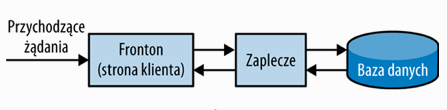
\includegraphics[width=12cm]{Rysunki/Rozdzial1/architektura_trojwarstwowa}
		\caption{Schemat aplikacji trójwarstwowej. Źródło \cite{Folwer:2019}}	
		\label{fig:architekturaTroj}
	\end{figure}

Przykładowe zaplecze oparte~o technologię \textit{LAMP} (ang. \textit{Linux-Apache-MySQL-Perl/PHP/Python)}\cite{Ziade:2018} dla każdej akcji przesłanej przez formularz \textit{HTML} generuje dużą ilość zapytań \textit{SQL} do bazy, a następnie odsyła nowo wygenerowaną stronę uaktualnioną~o żądane informacje\cite{Wilton:2005}. Twórcy takich serwisów zauważyli elementy stałe~w działaniu dla każdego~z nich. Dlatego naturalnym etapem rozwoju takich systemów było opracowanie ogólnodostępnych \textit{frameworków}, czyli zestawu narzędzi~i bibliotek służących do tworzenia podstawy aplikacji. Chcąc przewidzieć jakie problemy napotka programista stosowalni oni ujednolicone architektury, nie tylko jeżeli chodzi~o wzorce programowania, ale też~o cały system, począwszy od kontaktu~z bazą danych, działaniem serwera, sposobu generowania warstwy prezentacji, aż po zarządzaniem wydawania aplikacji~i jej serwowaniem użytkownikom końcowym. Obecnie standardem są dwa główne podejścia, monolityczne~i te oparte~o mikrousługi.

\section{Podejście monolityczne}
Monolit znaczy jednolity blok kamienny\footnote{Źródło: Słownik Języka Polskiego PWN \url{https://sjp.pwn.pl/sjp/monolit;2568347.html}}. Słowo to idealnie oddaje charakter tego typu architektury. Większość takich aplikacji została napisana~w oparciu~o model trójwarstwowy. Z tym, że \textit{fronton}\footnote{Warstwa prezentacji, również nazywana \textit{frontendem}.} (rys. \ref{fig:architekturaTroj}) i zaplecze mają wspólną bazę kodu. Umieszczone są we wspólnym repozytorium~i uruchamiane za pomocą jednego pliku wykonywalnego\cite{Folwer:2019}.

W książce \textit{Rozwijanie mikrousług~w Pythonie}, \textit{Tarek Ziadé} opisuje taką aplikacje na przykładzie agregatora hoteli\cite{Ziade:2018}. Omawiana strona posiada napisaną warstwę prezentacji~w statycznie generowanym \textit{HTML-u}. Użytkownik wchodząc na stronę przesyła zapytania \textit{SQL} do scentralizowanej aplikacji, która następnie prosi zewnętrzne usługi~o listę hoteli. Podczas rejestrowania miejsca~w hotelu kupujący otrzymuje stronę na którą musi się zalogować. Po przesłaniu danych~o płatności serwer komunikuje się~z usługą bankową zewnętrznego dostawcy, następnie informacje~o zakończonej transakcji przekazuje do bazy danych. Aplikacja sprawdza, czy wpis~o zakończeniu płatności jest już zapisana~w usłudze \textit{SQL}, jeśli tak, to na podstawie bazy danych generuje plik \textit{PDF} i przy pomocy \textit{usługi e-mail} przesyła potwierdzenie do użytkownika, sprawdzając jednocześnie informację~o wybranym przez niego hotelu~i również do niego kieruje powiadomienie email~z potwierdzeniem transakcji.

\begin{figure}[h!]
	\centering
		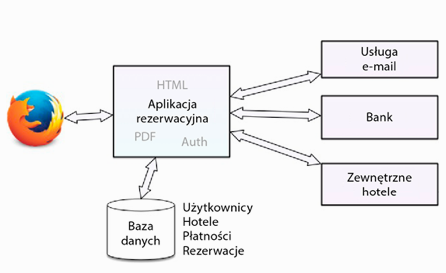
\includegraphics[width=10cm]{Rysunki/Rozdzial1/scentralizowanaArchitektura.png}
		\caption{Schemat scentralizowanej usługi rezerwującej miejsca~w hotelu. Źródło \cite{Ziade:2018}}
		\label{fig:scentralizowanaArchitektura}
\end{figure}

Z opisu jasno wynika, że każda interakcja użytkownika musi mieć swoją odpowiedź idącą~z aplikacji zarządzającej rezerwacjami. Nawet jeśli potrzebuje ona informacji, które bezpośrednio można byłoby otrzymać~z usług zewnętrznych. Tak samo dodatkowe serwisy, odsyłają informację zwrotną jedynie przez aplikacje centralną. Ten przykład dobrze przedstawia idee podejścia monolitycznego, centralnej usługi, która posiada~w sobie wiele przeróżnych funkcji, takich jak autentykacja, generowanie statycznych stron, a nawet plików \textit{PDF}. Wszystkie one są dostępne~w ramach jednej aplikacji, jednolitego bloku kamienia.

\subsection{Założenia aplikacji monolitycznej}
W tego typu aplikacji cała logika zawarta jest~w minimalnie jednym projekcie, który kompilowany jest pojedynczo, a następnie wdrażany jest jako całość. Oddzielanie poszczególnych problemów następuje poprzez grupowanie ich~w osobnych folderach, które~w miarę możliwości powinny izolować dane części aplikacji na \textit{warstwy logiczne}\cite{msbuild}. Założeniem jest wyodrębnienie struktur, które można ponownie używać~w ramach całej aplikacji. Wedle zasady \textit{DRY}\footnote{DRY (ang. \textit{Don't Repeat Yourself}) zasada zalecająca jak najmniejszą powtarzalność tych samych fragmentów kodu~w różnych miejscach aplikacji\cite{hunt:2011}.}. Dodatkowym atutem jest możliwość wymuszania ograniczeń~w sposobie komunikowania się pomiędzy poszczególnymi warstwami, dzięki hermetyzacji kodu\cite{msbuild}. Podstawy podejścia \textit{monolitycznego} są zbudowane na tych samych założeniach, co programowanie obiektowe\cite{Rodger:2019}. Organizacja kodu następuje poprzez hierarchię klas~i \textit{interfejsów}\footnote{W programowaniu obiektowym \textit{interfejsy} odpowiadają za definicję dla grup powiązanych funkcji, które klasa musi zaimplementować\cite{msbuild}.}. Daje to możliwości tworzenia różnych sposobów komunikacji pomiędzy poszczególnymi warstwami~i łatwiejszego wdrażania nowych funkcji. 

\subsection{Architektura aplikacji monolitycznej}
Warstwy logiczne są powszechnie używane przy tworzeniu aplikacji monolitycznych, dlatego powstało wiele technik pozwalających na ich organizację\cite{msbuild}. Najpopularniejszą~z nich jest podzielenie warstw aplikacji na te, które będą odpowiadać za dostęp do danych (\textit{Data Access Layer}), ich zarządzeniem (\textit{Business Logic Layer}) i interakcje~z użytkownikiem (\textit{User Interface}).
\begin{figure}[h!]
	\centering
		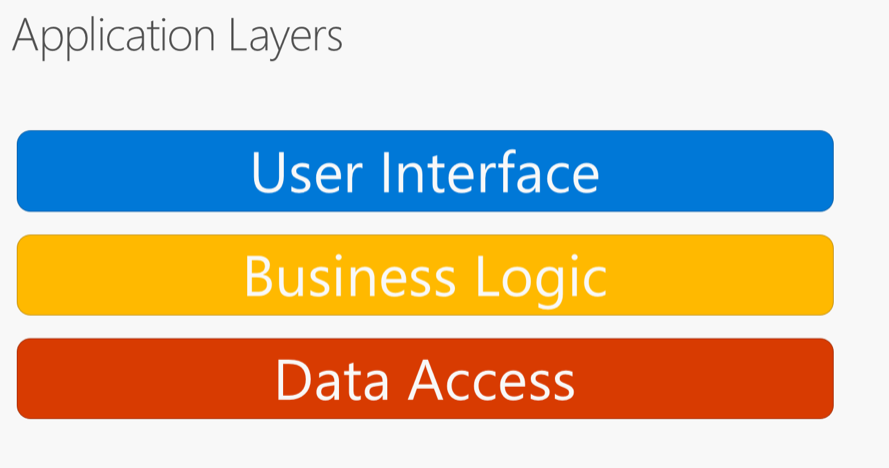
\includegraphics[width=9cm]{Rysunki/Rozdzial1/warstwyAplikacji.png}
		\label{fig:warstwyAplikacji}
	\caption{Struktura warstw aplikacji internetowej. Źródło \cite{msbuild}}
\end{figure}

Dzięki tej architekturze izoluje się możliwości interakcji~z poszczególnymi elementami aplikacji. Użytkownicy wchodzą~w interakcje jedynie~z warstwą \textit{UI}, która następnie współdziedziczy pewne elementy jedynie~z logiką biznesową, gdy zachodzi taka potrzeba, to ona komunikuje się~z warstwą odpowiedzialną za dostęp do bazy danych. Daje to gwarancję, tego, że każda część aplikacji zna dobrze swoje kompetencje~i ogranicza je jedynie do tych, za które jest odpowiedzialna\cite{msbuild}.

Współczesne \textit{frameworki} jeszcze bardziej rozdrabniają poszczególne warstwy, tak, aby udostępnić jedynie programistom \textit{interfejsy} za pomocą, których będą mogli tworzyć swoje aplikacje. \textit{Ruby on Rails} jest oparte~o architekturę \textit{MVC} (ang. \textit{Model-View-Controller}), gdzie modele, są klasami odpowiedzialnymi za interakcję~z dostarczonym przez \textit{framework} mechanizmem kontaktowania się~z bazą danych (\textit{ORMem}\footnote{ORM (ang \textit{Object-Relational Mapping}) system służący za odwzorowanie struktur bazodanowych na struktury programowania obiektowego, tak, aby uprościć tworzenie~i dostęp do bazy danych.}). Kontrolery, których zadaniem jest przyjmowanie danych od użytkownika, modyfikowanie modelu oraz odświeżanie widoków. Natomiast widoki, są odpowiedzialne za wygenerowanie szablonów \textit{HTML} i przesłanie ich do klienta aplikacji (przeglądarki użytkownika)\cite{ruby}.

Jedną~z odnóg architektury \textit{MVC} zastosowano~w \textit{frameworkach} napisany~w języku \textit{Python}, takich jak \textit{Django} i \textit{Flask}. Ich twórcy stworzyli je~w oparciu~o wzorzec \textit{MVT} (ang. \textit{Model-View-Template})\cite{django}, nie różni się on bardzo od pierwowzoru, z tą różnicą, że zamiast klas generujących pliki \textit{HTML}, jego twórcy stworzyli moduł odpowiedzialny za przetwarzanie tego rodzaju plików posiadających specjalne znaczniki (na przykład \textit{Jinja2}\footnote{Więcej~o składni \textit{Jinja2} pod adresem \url{https://jinja.palletsprojects.com/en/2.11.x/}.}). Dostarczają one dodatkowej logiki do interakcji~z danymi przesłanymi przez widok.

\begin{lstlisting}[caption={Przykład szablonu \textit{Django}. Plik \textit{index.html}. Żródło \cite{django}}] 


{{ section.title }}


<h1>{{ section.title }}</h1>


<h2>
  <a href="{{ story.get_absolute_url }}">
    {{ story.headline|upper }}
  </a>
</h2>
<p>{{ story.tease|truncatewords:"100" }}</p>


\end{lstlisting}
Istnieje jeszcze wiele innych podejść do projektowania monolitycznych aplikacji internetowych, te przedstawione tutaj są jednymi~z najpopularniejszych. Jak widać struktury zaprezentowanych \textit{frameworków} internetowych są mocno powiązane~z wcześniej opisanym modelem trójwarstwowym (rys. \ref{fig:architekturaTroj}).

\section{Mikrousługi}
Opozycją do podejścia gdzie, jedna centralna aplikacja, komunikuje się~z zewnętrznymi usługami jest stworzenie kilku mniejszych działających osobno programów. Ich kod można by było podzielić na kilka oddzielnie uruchamianych procesów, które mają odmienne mniejsze zadania do zrealizowania\cite{Ziade:2018}. Wracając do przykładu agregatora hoteli podanego przez \textit{Tarek Ziade}, zamiast jednej usługi odpowiedzialnej za komunikację, generowanie plików, obsługę banku~i e-maili, można byłoby stworzyć wiele mniejszych \textit{mikrousług}.
	
\begin{figure}[h!]
	\centering
		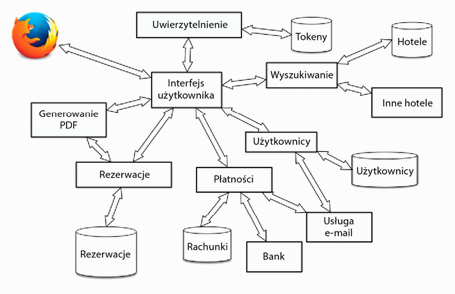
\includegraphics[width=12cm]{Rysunki/Rozdzial1/mikrouslugi}
		\caption{Schemat scentralizowanej aplikacji~z rys. \ref{fig:scentralizowanaArchitektura} oparty~o architekturę mikrousług. Źródło \cite{Ziade:2018}}	
		\label{fig:mikrouslugi}
	\end{figure}
	
Autor książki \textit{Rozwijanie mikrousług~w Pythonie} z powyższego schematu (rys.~\ref{fig:mikrouslugi}), wyodrębnia 7 niezależnych komponentów\cite{Ziade:2018}, takich jak:

\begin{enumerate}
  \item \textbf{Interfejs użytkownika}: frontalną usługę zajmująca się generowaniem \textit{HTMLa} i komunikacją~z innymi procesami.
  \item \textbf{Wyszukiwanie hoteli}: program tworzący listę hoteli na podstawie danych~z zewnętrznych usług.
  \item \textbf{Użytkownicy}: usługa mająca na celu zarządzanie bazą użytkowników~i wysyłaniem do nich wiadomości e-mail.
  \item \textbf{Rezerwacje}: proces odpowiedzialny za zarządzeniu danymi na temat rezerwacji, a także przesyłaniem ich do generatora \textit{PDFów}.
  \item \textbf{Generator PDF}: program generujący na podstawie szablonów~i danych odpowiednio sformatowane pliki \textit{PDF}.
  \item \textbf{Płatności}: moduł komunikujący się~z zewnętrzną usługą banku, również zapisuje informacje~o płatnościach~i wysyła je użytkownikowi~w wiadomości email.
  \item \textbf{Uwierzytelnianie}: usługa generująca \textit{tokeny} stosowane przez inne procesy do uwierzytelniania użytkowników.
 \end{enumerate}
 
 Powyższe mikrousługi mają tą samą funkcjonalność, co aplikacja monolityczna~z rys. \ref{fig:scentralizowanaArchitektura}. Jednak do komunikacji nie wykorzystują elementów programowania obiektowego, a odpowiedni do tego protokół. W tym kontekście każda usługa stanowi osobną logiczną jednostkę odpowiedzialną za jedno ściśle określone zadanie\cite{Ziade:2018}. Takie niezależne usługi nazywane są również komponentami.
  
\subsection{Założenia mikrousług}
Podejście~z wykorzystaniem mikrousług oparte jest~o niewielkie komponenty, które komunikują się~z sobą~w ten sam jednolity sposób bez żadnych przeszkód\cite{Rodger:2019}. \textbf{Niezależnie od warstwy transportowej}, to znaczy, że dane dwie usługi nie muszą nawet wiedzieć~o swoim istnieniu, aby jedna zastąpiła drugą~w przenoszeniu informacji\cite{Rodger:2019}. Wystarczy, że otrzymują~i zwracają odpowiednie komunikaty. Dlatego ważne jest, aby wewnątrz nich znajdowały się informacje~o tym jakie wartości powinny być~w wiadomości zwrotnej, ta cecha to \textbf{dopasowanie do wzorca}. Daje ona możliwość dynamicznego definiowania~z jakiej pomocy innej mikrousługi może skorzystać ta, która obecnie przetwarza informację. Najczęściej~w tym celu stosuje się protokół \textit{HTTP}\cite{http} oparty~o architekturę \textit{REST} (ang. \textit{Representational state transfer}), mającą za zadanie zunifikować odbierane~i wysyłane żądania~w zależności od ich treści\cite{Rodger:2019}. W niezależnych od języka programowania formatach takich jak \textit{JSON}, \textit{XML}, czy \textit{YAML}\cite{Ziade:2018}.

Osiągnięcie pełnej uniwersalności komunikatów nie jest możliwe. Wspomniane wcześniej wzorce muszą być zdefiniowane przez programistów~w ramach architektury \textit{REST}. Każda usługa powinna udostępniać \textit{API} (ang. \textit{Application Programming Interface}), czyli interfejsy, które pomogą innym programistom dostosować się do wzorca komunikatów dla danej usługi\cite{Ziade:2018, Rodger:2019}. To na zespole zajmującym się określony mikroserwisem spoczywa odpowiedzialność za dobrze udokumentowanie \textit{API}, wówczas nie musi się on przejmować wyborem języka programowania, \textit{frameworków}, czy bazy danych\cite{Ziade:2018}.

\begin{figure}[h!]
	\centering
		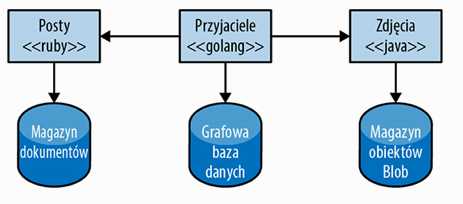
\includegraphics[width=10cm]{Rysunki/Rozdzial1/rozneTechnologie.png}
		\caption{Schemat prezentujący zastosowanie różnych technologii do budowania aplikacji opartych~o mikroserwisy. Źródło \cite{Newman:2016}}	
		\label{fig:rozneTechnologie}
	\end{figure}
	

Z zasady każda usługa powinna być niewielka, ponieważ ma ona ściśle określone cele, a~w razie, gdy będą potrzebne nowe funkcje dla całego systemu, to będzie je można bez przeszkód wprowadzić dodając niezależną jednostkę. Ta charakterystyczna dla mikrousług cecha, to \textbf{addytywność}. Pomaga to~w zapewnieniu dużego~i bardzo skomplikowanego systemu (jako zbioru wszystkich mikrousług) bez większego długu technicznego\cite{Rodger:2019}. W razie potrzeby dowolna jego część jest wymieniana~i zastępowana, bez żadnego ryzyka niestabilnego działania całości aplikacji. Co~w praktyce powinno przekładać się na dużą skalowalność projektu~i jego łatwe wdrożenie\cite{Ziade:2018}.

\subsection{Architektura mikrousług}
Nie ma jednego wzorca pozwalającego określić budowę całego systemu opartego na mikrousługach. W przeciwieństwie do aplikacji monolitycznych, małe niezależne serwisy nie wymagają dogłębnego projektowania hierarchii klas, czy zależności pomiędzy poszczególnymi modułami. W tym wypadku najważniejsze jest spojrzenie na cały system od strony komunikatów, a nie~z perspektywy poszczególnych komponentów. Łatwiej wówczas analizować sposoby interakcji pomiędzy nimi, znajdować odpowiednie wzorce~i dobrze dostosować ich architekturę\cite{Rodger:2019}. Taki pogląd na sytuacje uświadamia, że~w przypadku mikrousług najważniejsze jest dobre zaprojektowanie warstwy transportowej. Wiedza, że poszczególna usługa, to tak naprawdę osobny mini serwer \textit{HTTP} pozwala zwrócić uwagę na ważną cechę~i zarazem niebezpieczeństwo takich jednostek, czyli potrzebę znajomości lokalizacji innej zależnej mikrousługi. W tym celu powinien zostać zaprojektowany proces pozwalający na odnajdowanie innych aplikacji. Rodzi to szereg problemów, ponieważ utrzymywanie takiej usługi nie jest proste, a napisanie dobrej implementacji jest zdaniem dość trudnym\cite{Rodger:2019}. Kolejną sprawą jest to, że przy takim układzie, mikrousługi muszą przechowywać szczegółową wiedzę~o konkretnych serwisach, a to prowadzi do ścisłych zależności. Właśnie tutaj widać fundamentalną różnicę między architekturą mikrousług, a monolitu. Żeby jednolita centralna aplikacja~w którymś~z modułów skorzystała~z metody danej klasy ważne jest, aby posiadała do niej referencję. Z mikrousługami jest podobnie, z tą różnicą, że wszystko odbywa się przez sieć. Dana usługa korzysta~z informacji~o lokalizacji innego serwisu, a także odpowiedniego adresu \textit{URL}, aby skorzystać~z możliwości kolejnej. Odpowiednie zaprojektowanie tej komunikacji ogranicza potrzebę dostarczania dodatkowych usług~i kodu, którego zadaniem byłoby współpracowanie~z mechanizmem wykrywania poszczególnych modułów\cite{Rodger:2019}.
\newpage
W najprostszej konfiguracji mikrousługi komunikują się~z sobą bezpośrednio, ale warto rozszerzyć tą architekturę~o moduły równoważenia obciążenia protokołu \textit{HTTP}, tak zwane \textit{load balancery}. Pozwala to na obsługiwanie ruchu dla różnych instancji mikrousług, a także zapewni proste skalowanie tych usług\cite{Rodger:2019}. Niestety, zwiększy to również złożoność wdrażania takiego systemu.

 \begin{figure}[h!]
	\centering
		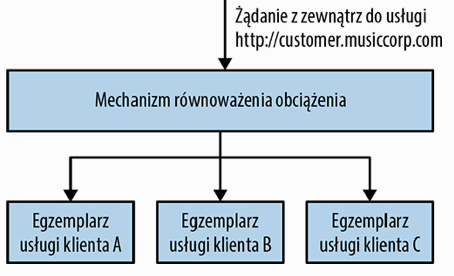
\includegraphics[width=10cm]{Rysunki/Rozdzial1/rownowazenieObciazenia.png}
		\caption{Schemat prezentujący zastosowanie mechanizmu do skalowania liczby instancji usługi klienta. Źródło \cite{Newman:2016}}	
		\label{fig:rownowaznieObciazenia}
	\end{figure}
	
Za jednym \textit{load balancerem} mogą stać różne usługi, ogranicza to czas ich wdrożenia, koszty~i zbędne konfiguracje, ale również może się okazać wąskim gardłem~w działaniu systemu. To~w jaki sposób zostanie wykorzystane narzędzie równoważenia obciążenia zależy od architekta aplikacji~i ma duże znaczenie~w jej działaniu. Ważne jest znalezienie optymalnej konfiguracji~i pokrycie odpowiednich serwisów.
	
\chapter{Projekt aplikacji}
\label{roz3}
%=================================================================================================
Do porównania budowy aplikacji stworzonych~w oparciu~o podejście monolityczne~i mikrousługi wykorzystane będą dwa serwisy. Obie platformy będą miały taką samą funkcjonalność, tak, aby porównanie ich było jak najbardziej miarodajne. W tym celu zostaną również wykorzystane, gdzie tylko to możliwe, te same technologie~i \textit{frameworki}. Oczywiście, charakterystyka obu podejść będzie wymagała, żeby niektóre obszary aplikacji znaczenie się od siebie różniły, ale będą to jedynie elementy konieczne do realizacji założeń danej architektury.

\section{Opis projektu}
W ramach projektu stworzona zostanie prosta aplikacja do dodawania zadań. Po wejściu na stronę internetową użytkownik będzie mógł się do niej zarejestrować lub zalogować, a następnie ukaże mu się widok listy, służący do przeglądania aktualnych celów. Serwis pozwalać będzie na dodawania nowych zadań, ich aktualizację, a także usuwanie. Możliwe będzie również odznaczenie danego celu jako zrealizowany. Po skorzystaniu~z aplikacji będzie można się~z niej wylogować.

%=================================================================================================
\section{Założenia projektowe}
Głównym założeniem projektu było stworzenie dwóch niewielkich aplikacji, które mogłyby~w pełni zobrazować idee obu wspomnianych podjeść. Istotne jest przedstawienie procesu tworzenia architektury takich aplikacji~i ich implementacji, a nie opracowanie skomplikowanych systemów posiadających ogromną ilość funkcji. To oczywiście jest celem biznesowym każdego realnego projektu informatycznego, ale założeniem pracy jest głównie porównanie takich usług, a nie ich całkowita realizacja~i wdrożenie. Nie mniej jednak te aplikacje posiadać będą podstawowe elementy do ich przetestowania, takie jak mechanizm przesyłania stron internetowej do klienta, interfejs użytkownika, część odpowiedzialną za zarządzanie danymi, a także bazę danych, która będzie je przechowywać. Ważne~z projektowego punktu widzenia będzie zaimplementowanie odpowiedniej komunikacji na poziomie poszczególnych komponentów aplikacji. W systemie monolitycznym będzie to zadbanie~o dobrą strukturę projektu~i stworzenie hierarchii klas, tak, aby zapewnić modułom odpowiedni poziom izolacji~i ich logiczny podział. W przypadku mikrousług głównym założeniem będzie stworzenie interfejsu komunikacji opartego na dostarczeniu \textit{API} przez poszczególne komponenty, a także opracowanie sposobu pozwalającego na łączenie się między sobą dwóch usług. Ważne będzie ograniczenie działania tych jednostek do obsługi konkretnego zadania.

Do zarządzania tymi systemami wykorzystane zostanie narzędzie odpowiedzialne za konteneryzacje, tak aby zapewnić aplikacjom niezawodność działania niezależnie od platformy, a także ułatwić ich zarządzanie~i wdrażanie. Szczególnie~w systemach opartych~o mikrousługi wykorzystanie takiego narzędzia usprawnia ich rozwój, ponieważ cały system jest konfigurowany raz, a pomimo tego działa~w ten sam sposób na wielu hostach.

Następnym elementem projektu jest przedstawienie procesu testowania obu platform, porównania ich właściwości, a także przedstawienie możliwości integracji~z usługami dostarczającymi infrastrukturę serwerową. Wskazane zostaną różnice pomiędzy dwoma tymi podejściami na każdym~z wymienionych wcześniej etapów.

Ostatnim elementem projektu będzie analiza obu podejść, wskazanie ich wad~i zalet. Znalezienie przypadków, dla których najlepiej sprawuje się dana architektura, tak, aby czytelnik, który~w przyszłości tworzyłby serwis internetowych, był świadomy korzyści~i konsekwencji płynących~z wyboru jednego~z opisanych podejść.

\section{Opis problemu~i dostępnych rozwiązań}
\label{sec:problemy}
Problemem przy tworzeniu dwóch aplikacji internetowych opartych~o różne podejścia co do architektury całego sytemu, a zarazem muszących być pod względem technologicznym do siebie podobne, jest znalezienie uniwersalnego narzędzia do tworzenia takich usług. Istnieje wiele \textit{frameworków} pozwalających na budowanie serwisów internetowych, ale tylko część~z nich zapewnia odpowiedni poziom uniwersalności, tak, aby nie faworyzować jednej~z dostępnych architektur. Na przykład \textit{Django} zostało opracowane głównie tak, aby tworzyć serwisy monolityczne, przy generowaniu projektu powstaje już odpowiednia do tego struktura\footnote{Opis tworzenia nowego projektu~i generowania jego struktury został szczegółowo opisany~w pierwszym rozdziale dokumentacji \textit{frameworku}. Link do niej - \url{https://docs.djangoproject.com/en/3.0/intro/tutorial01/}.} z wygenerowanymi szablonami~i panelem admina. Dzięki istnieniu bibliotek takich jak \textit{Django Rest Framework}\footnote{Link do projektu \url{https://www.django-rest-framework.org}.} można zmienić strukturę aplikacji~i zaimplementować~w niej \textit{API} wysyłające komunikaty zgodnie~z założeniami \textit{REST}, ale polega to na wielu zmianach konfiguracji~i doinstalowaniu kilku narzędzi. Szczególnie, że \textit{Django} domyślnie posiada wiele modułów~i jest stosunkowo dużym frameworkiem\footnote{Wszystkie narzędzia~i funkcje, które posiada \textit{Django} są szczegółowo opisane~w dokumentacji. Link \url{https://docs.djangoproject.com/en/3.0/}.}.

Z drugiej strony istnieją biblioteki głównie zorientowane~i przystosowane na dostarczanie \textit{REST API}. Są to minimalistyczne \textit{frameworki} w których najważniejsza jest ich mała waga, brak wielu zależności~i duża szybkość, takim przykładem jest \textit{Falcon}\footnote{Szczegółowo idea \textit{Falcona} została przedstawiona~w jego dokumentacji pod adresem \url{https://falcon.readthedocs.io/en/stable/index.html}.}.

Na szczęście istnieją narzędzia pozwalające na łatwą implementację zarówno jednolitej aplikacji jaki~i minimalistycznej usługi skierowanej na wykonanie poszczególnego zadania, serwującej \textit{API} oparte~o \textit{REST}. Nie wymaga to usuwania dużej ilości zależności instalowanych wraz~z generowaniem projektu, a także całkowitego przepisywania istniejących konfiguracji. Taką biblioteką jest \textit{Flask}. Jego twórcy opisują go jako \textit{mikroframework}, co oznacza, że całą aplikację można napisać~w jednym pliku bez utraty jakichkolwiek funkcji, a rdzeń narzędzia jest utrzymywany jako maksymalnie mały~i możliwy do rozbudowania przez korzystającego~z niego programistę\cite{flask}. Biblioteka ta ma dużą bazę dodatków rozszerzających funkcję tworzonej~w niej aplikacji, które~w łatwy sposób można~z nią zintegrować\cite{flask}. Rozszerzenia te pozwalają na dodanie takich narzędzi jak integracje~z różnymi bazami danych, obsługa wysyłania plików, czy integracja~z bibliotekami do autentykacji\footnote{Więcej szczegółów zostało opisanych~w dokumentacji. Link \url{https://flask.palletsprojects.com/en/1.1.x/foreword}.}. Framework pomimo swojej małej wielkości nadaje się do szerokiego zastosowania\cite{flask}.

Ta biblioteka sprawdzi się również, w ramach opisywanego wcześniej problemu, do tworzenia dużych aplikacji. Posiada ona dodatki do obsługi różnych baz danych, system \textit{ORM}\footnote{Link do jego dokumentacji \url{https://flask-sqlalchemy.palletsprojects.com/en/2.x/}.} pozwalający na stworzenie klas \textit{modeli}, narzędzia do zarządzania logiką aplikacji, nadawania im poszczególnych adresów (funkcje za które odpowiedzialny są widoki, (ang. \textit{view})) i wysyłania odpowiedzi~w formacie \textit{JSON} lub generowania szablonów \textit{HTML} (\textit{templates}) na podstawie przesłanych do nich danych przy pomocy składni \textit{Jinja2}\cite{flask}. Z tego powodu \textit{Flask} zapewnia dostateczne możliwości do tworzenia dużych monolitycznych aplikacji jaki~i małych mikrousług.

Kolejnym problemem, który należałoby rozwiązać na etapie projektowania specyfikacji technicznej aplikacji jest warstwa prezentacji. W podejściu opartym~o mikrousługi powinna to być osobna niezależna jednostka mogąca działać nawet bez konieczności uruchamiania innych usług. Istnieje rozwiązania oparte~o \textit{runtime} silnika \textit{V8} przeglądarki \textit{Google Chrome}, czyli narzędzie \textit{Node.js}\footnote{Link do dokumentacji \textit{Node.js}, \url{https://nodejs.org/en/}.}. To pozwoliło na powstanie progresywnych \textit{frameworków webowych} do budowania interfejsu użytkownika\cite{vuejs}. Wykorzystują one wcześniej wspomniany \textit{runtime} do tworzenia \textit{virtual DOMa}, czyli struktury \textit{HTML'u} czytanej już bezpośrednio przez przeglądarkę klienta, ale zarządzanej przez język \textit{JavaScript}, co ma przekładać się na łatwość obsługi jej poszczególnych elementów, aktualizowania lub sterowania ich stanem\cite{vuejs}. Dodatkowo takie \textit{frameworki} posiadają skrypty do generowania gotowych projektów, gdzie dostarczają proste serwery, które pozwalają na przeładowywanie strony przy każdej zmianie pliku. Opisywaną bibliotekę można również dołączyć do statycznego pliku \textit{HTML}, co przyda się przy tworzeniu aplikacji monolitycznej. Większość~z tych narzędzi manipuluje kodem strony jedynie przez język \textit{JavaScript}\cite{vuejs}. Natomiast biblioteka \textit{Vue.js} pozwala na to za pomocą kodu \textit{HTML} i specjalnej składni (podobnej do \textit{Jinja2}), dzięki czemu~o wiele łatwiej jest tworzyć taką aplikację wewnątrz pliku \textit{HTML}. Z kolei nowoczesne przeglądarki posiadają narzędzia do pobierania~i wysyłania zasobów takie jak \textit{Fetch API}\cite{mdn}. Pozwala to na obsługę zapytań \textit{HTTP}\footnote{Więcej informacji~o działaniu~i posługiwaniu się \textit{Fetch API} można znaleźć dokumentacji zasobów internetowych fundacji \textit{Mozilla}. Link \url{https://developer.mozilla.org/en-US/docs/Web/API/Fetch_API/Using_Fetch}.} po stronie klienta już po przesłaniu mu wygenerowanego pliku \textit{HTML}, jest to więc sposób na komunikację między usługą interfejsu użytkownika, a pozostałymi mikrousługami działającymi po stronie serwera.

Istnienie wielu powiązanych~z sobą usług lub nawet jednej centralnej aplikacji wiąże się~z dużą ilością potrzebnych do uruchomienia zależności, konfiguracji, a nawet warstwy sprzętowej\cite{Ziade:2018}. Dlatego dobrym rozwiązaniem jest zastosowanie \textit{maszyny wirtualnej}, programu symulującego środowisko danego sprzętu, wraz~z jego systemem. Niektóre duże projekty zostały nawet przeniesione jako gotowe obrazy takich \textit{maszyn wirtualnych}. Dzięki czemu udało się je spakować wraz~z wypełnionymi bazami danych do uniwersalnych formatów, które bez żadnej konfiguracji można uruchomić za pomocą jednego polecenia\cite{Ziade:2018}. Niestety, takie rozwiązania często są płatne~i ze względu na potrzebę dużej mocy obliczeniowej trudno jest je stosować~w środowisku produkcyjnym\cite{Ziade:2018}. Rewolucją okazał się \textit{Docker}, otwarta platforma do konteneryzacji. W odróżnieniu od wcześniej wspomnianych metod \textit{Docker} nie stara się symulować całego sprzętu, a jedynie odizolować środowisko za pomocą wysokopoziomowych narzędzi wykorzystywanych~w systemie \textit{Linux}. Projekt zbudowany za pomocą tej platformy jest~w stanie działać~w każdym środowisku bez względu na system operacyjny~z zachowaniem normalnej prędkości działania\cite{Ziade:2018}, a dzięki usłudze \textit{Docker Compose} można dostarczyć do projektu plik~z konfiguracją\cite{docker} całego procesu jego uruchomienia za pomocą narzędzia \textit{Docker}, co~w efekcie pozwoli na wystartowanie projektu wykorzystując jedną prostą komendę. Wystarczy mieć na komputerze zainstalowaną omawianą platformę\footnote{Link do instrukcji zainstalowania \textit{Dockera} i \textit{Docker-compose}, \url{https://docs.docker.com/get-docker/}.}.

Niezależnie od tego, czy obsługujemy duży połączony~z sobą system wielu usług, czy też jedną centralną aplikację potrzebne będzie usługa \textit{serwera WWW}. W przypadku monolitu obsługuje on zapytania \textit{HTTP} na poziomie systemu, nasłuchując na zapytania zewnątrz~i przekazując te odpowiedzi (serwer \textit{Proxy}\cite{nginx}) do~i~z serwera \textit{uWSGI} \textit{Flaska}, wówczas można byłoby zastosować usługę \textit{Nginx}\cite{flask}, lub też skorzystać~z gotowych rozwiązań, takich jak chmura \textit{AWS}, \textit{Heorku}, \textit{Azure}, \textit{PythonAnywhere}\cite{flask}. W przypadku mikrousług, które będą wewnątrz kontenera to, potrzebny będzie proces odpowiedzialny za wewnętrzną komunikację, a także \textit{load balancer}. Wszystkie te opcje również udostępnia \textit{Nginx}\cite{nginx}.

%=================================================================================================
\section{Architektura systemu}
Zgodnie~z głównym założeniem pracy~w jej ramach przedstawione zostaną dwie aplikacje oparte~o różne podejścia, monolityczne~i mikrousługi. Każda~z nich wymaga odmiennego spojrzenia na ich budowę~i architekturę. Odmiennego zaprojektowania hierarchii klas~i warstwy transportowej dla przetwarzanych danych.
\subsection{Podejście monolityczne}
Architektura aplikacji monolitycznej została zorientowana~o wcześniej opisany wzorzec \textit{MVT}. Zakłada on wykorzystanie hierarchii obiektów dostarczony przez \textit{framework} do zbudowania komponentu opartego~o \textbf{modele}, czyli klasy odpowiadającej za dostarczenie odpowiednich struktur~i relacji~w bazie danych. Następnie za pomocą \textit{ORMa}, który posiada zestaw narzędzi do tworzenia kwerend, dostarczone będą dane przetwarzane~w warstwie \textbf{widoków}. Ich rola nie tylko sprowadza się do interpretowania przesłanych informacji~i odsyłania ich klientowi. Odbywa się~w nich również dopasowywanie (\textit{routing}) zapytań do funkcji~i metod, które je przetwarzają~i zwracają jako wygenerowane \textbf{szablony}. 

Na schemacie poniżej (rys. \ref{fig:architekturaMono}) jest strzałka zwrotna~z przeglądarki do szablonu. Użytkownik dostając wygenerowany kod \textit{HTML} wykorzystuje zawarte~w nim formularze do wysłania danych do widoku. Możliwe jest ich bezpośrednie wysłanie, ale polega to na odtworzeniu odpowiedzi serwera.
\begin{figure}[h!]
	\centering
		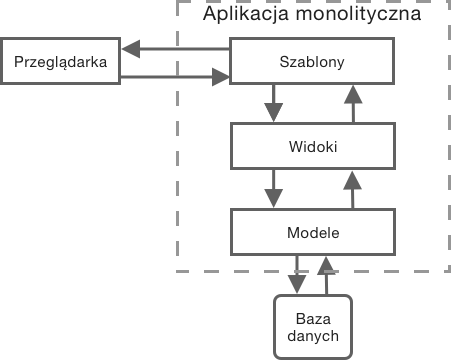
\includegraphics[width=12cm]{Rysunki/Rozdzial3/architekturaMono}
		\caption{Schemat architektury monolitycznej.}	
		\label{fig:architekturaMono}
	\end{figure}

\subsection{Mikrousługi}
Architektura mikrousług będzie zakładała, że jedna centralna aplikacja zostanie rozbita na mniejsze działające osobno. W celu porównania obu serwisów baza danych nie będzie dzielona na mniejszą, tak aby to nie zapis~i odczyt do niej był decydującym czynnikiem wskazującym na wyższość jednego~z rozwiązań, ale będzie korzystać~z różnych baz jednej usługi.

Aplikacja zarządzająca listami zadań posiadałaby cztery podstawowe moduły. Pierwszy~z nich \textbf{interfejs użytkownika}, który za pomocą dostarczanego~z przeglądarką \textit{Fetch Api}\cite{mdn} kontaktuje się~z resztą aplikacji. Użytkownik po wejściu na stronę główną przechodzi do zakładki logowania. Następnie informacje wymagane do zalogowania wpisuje~w formularz~i przesyła żądanie do usługi \textbf{użytkownicy}, zwraca ona dane użytkownika~z jego aktualnym \textit{tokenem}. Interfejs użytkownika sprawdza następnie jego poprawność~w jednostce \textit{autentykacja}\cite{Herman:2017}, gdy wszystko się zgadza klient dostaje ten sam \textit{token} z powrotem. Gdyby dany token istniał, ale jego termin ważności wygasł, to ta usługa jest odpowiedzialna za wygenerowanie nowego. Uzyskany klucz od tej pory służy do otrzymywania informacji zarezerwowanych jedynie dla zalogowanych użytkowników. Inną usługą są listy zadań, komponent ten odpowiada za zwracanie, tworzenie~i usuwanie, zadań dla poszczególnych ich właścicieli.
\begin{figure}[h!]
	\centering
		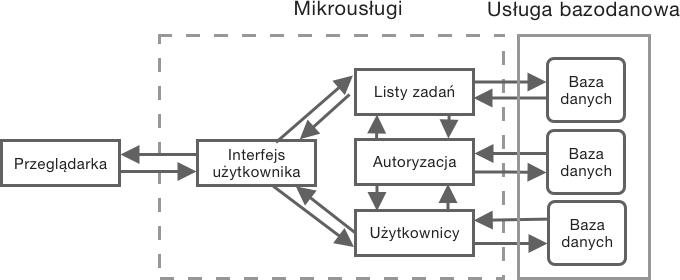
\includegraphics[width=14cm]{Rysunki/Rozdzial3/architekturaMirko.png}
		\caption{Schemat architektury mikrousług.}	
		\label{fig:architekturaMikro}
	\end{figure}

\section{Baza danych}
\label{sec:bazadanych}
Baza danych będzie posiadała dwie główne tabele: użytkownicy~i listy zdań. Będą one połączone za pomocą relacji \textit{one-to-many} w wielu \textit{frameworkach} nazywanej również kluczem obcym. Oznacza to, że jeden użytkownik będzie mógł mieć wiele zadań przypisanych do siebie, natomiast jedno zadanie będzie przypisane tylko do jednego użytkownika. Struktura ta szczegółowo została pokazana na schemacie poniżej.
\begin{figure}[h!]
	\centering
		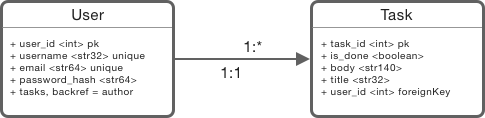
\includegraphics[width=12cm]{Rysunki/Rozdzial3/databaseSchema.png}
		\caption{Schemat bazy danych.}	
		\label{fig:schematbazydanych}
	\end{figure}
	
Jak można zauważyć na schemacie (rys.\ref{fig:schematbazydanych}), użytkownik posiada pole \textit{tasks}, które odpowiada za relację \textit{one-to-many} i tworzy referencję wsteczną\cite{Wilton:2005} dla modelu zadań~o nazwie \textit{author}, dzięki temu korzystając~z listy zadań nadal można mieć dostęp do informacji~o kliencie. Doprowadza to do potrzeby stworzenia pola \textit{user\_id} (klucza obcego) i ustanowienia relacji \textit{many-to-one} po stronie zadania.

Inną sprawą jest też, aby każdy użytkownik posiadał unikatowy \textit{username} i \textit{email}, tak żeby nie było sytuacji, w której wyciągając te informacje~z bazy danych, a następnie nimi operując nie wysłać emaila~z jakimiś wrażliwymi danymi do dwóch osób na raz. W bazie danych hasła użytkowników nie są zapisane zwykłym tekstem (ang. \textit{plain text}), ale są zatajone za pomocą funkcji haszującej (ang. \textit{hash function}). Domyślnie zestaw narzędzi \textit{Werkzeug} posiada odpowiednie metody spełniające standard \textit{PBKDF2} i wykorzystujące algorytm \textit{SHA-1} do szyfrowania haseł\cite{Ziade:2018}.

 
%=================================================================================================
\section{Wykorzystane biblioteki}
Ważne jest, aby aplikacja monolityczna, tak jaki~i te mniejsze mikrousługi oparte były~o ten sam zestaw technologii za nie odpowiedzialny. Dlatego większość wymienionych bibliotek będzie użytych~w obu projektach. W liście zostały uwzględnione tylko te główne pakiety. Wiele~z nich domyślnie instaluje mniejsze jako swoje zależności~i wypisanie ich wszystkich nie jest konieczne, aby zrozumieć działanie aplikacji. Lista najistotniejszych znajduje się poniżej:

\begin{itemize}
	\item \textit{Vue.js}\cite{vuejs}, biblioteka odpowiadająca za warstwę prezentacji.
	\item \textit{Flask}\cite{flask}, \textit{mikroframework} odpowiedzialny za usługę serwera \textit{HTTP}.
	\item \textit{Nuxt.js}\cite{nuxtjs}, framework do tworzenia progresywnych aplikacji oparty~o \textit{Vue.js}.
	\item \textit{Flask SQLAlechmy}\cite{flasksql}, system do zarządzania bazą danych~w ramach aplikacji napisanych we \textit{Flask}u. 
\end{itemize}
% TODO opisać więcej bibliotek


%=================================================================================================
\section{Analiza wymagań}
Tworzone na potrzebę pracy projekty powinny mieć zdefiniowane wymagania, tak aby jasne były konkretne ich cele do zrealizowania. Ma to zapobiec implementacji nadmiarowej ilości funkcji, a przy okazji wyszczególnić zestaw cech, które definiują projekt jako gotowy. W związku~z tym, że celem pracy jest porównanie dwóch architektur, to sam projekt nie musi działać jak pełnoprawny produkt, a jedynie posiadać wszystkie istotne elementy potrzebne do realizacji danej architektury~i możliwości porównania jej~z drugą.

\subsection{Wymagania funkcyjne}
Korzystając~z wspieranych przeglądarek internetowych (rozdział \ref{sec:przegladarki}), użytkownik powinien móc wejść na wskazany adres~i wczytać stronę główną projektu. Następnie klikając odnośnik \textit{login} na górnej belce serwisu, następuje przekierowanie do strony logowania, gdzie będzie możliwy wybór jednego~z dwóch formularzy, jeden do zalogowania już istniejącego użytkownika, a drugi do jego zarejestrowania. Po ich wypełnieniu~i przesłaniu następuje autentykacja, dzięki czemu osoba korzystające~z serwisu będzie mogła przeglądać utworzstone przez siebie zdania, tworzyć nowe~i je usuwać. Dodatkowo możliwe będzie określenie czy zadanie zostało wykonane. Powyżej listy celów będzie znajdował się przełącznik do wyświetlania zadań, które nie zostały skończone, a także tych które są gotowe. Szata graficzna strony będzie minimalistyczna, wyróżniać się będą różne rodzaje szarości. Po skończeniu korzystania~z strony użytkownik będzie mógł się~z niej wylogować, wówczas straci dostęp do listy zadań~i nie będzie mógł tworzyć nowych, ani edytować istniejących.

\subsection{Wymagania niefunkcyjne}
Istotą projektów jest sprawdzenie dwóch różnych podejść przy tworzeniu aplikacji internetowych. Ważne jest przetestowanie podstawowych funkcji, które oferują serwisy, takich jak logowanie użytkownika, tworzenie formularzy, wysyłanie zapytań: \textit{GET, POST, DELETE, UPDATE, PUT}\footnote{Podstawowe rodzaje zapytań dla standardu \textit{HTTP} \textit{REST}.} i komunikacja pomiędzy poszczególnymi komponentami serwera. Obie strony powinny posiadać również interfejs użytkownika, wraz~z skryptami~w języku \textit{JavaScript} i arkuszami styli \textit{CSS}.

Oba projekty będą wykorzystywać konteneryzację do spakowania ich~i łatwiejszego uruchomienia na maszynie programisty, prywatnym serwerze wirtualnym lub usłudze do serwowania serwisów internetowych.

\section{Środowisko programistyczne}
Obie aplikacje będą dzielić się na stronę serwerową~i warstwę prezentacji. Końcowy użytkownik do działania serwisu będzie potrzebował jedynie przeglądarki. Natomiast do uruchomienia serwera potrzebne będzie narzędzie odpowiadające za konteneryzację projektu.
 \subsection{Aplikacja serwera}
 Narzędziem wykorzystanym do konteneryzacji projektu jest \textit{Docker}, dzięki tej usłudze żadne inne zależności ani programy nie są wymagane. Należy jedynie pobrać program~z strony: \url{https://docs.docker.com/get-docker/} i~w zależności od zainstalowanego na komputerze systemu operacyjnego, odpowiednio przejść wszystkie kroki~w instalatorze.
 
 Po instalacji wystarczy, że usługa ta zostanie uruchomiona\footnote{Dla systemów~z rodziny \textit{Linux} konfiguracja jest nieco trudniejsza. Trzeba dodać jeszcze \textit{Dockera} do specjalnej grupy, aby przy każdym uruchomieniu nie używać praw administratora, \textit{sudo}. Opis procedury znajduje się na stronie \url{https://docs.docker.com/engine/install/debian/}. Dodatkowo należy stworzyć \textit{demon}, żeby narzędzie uruchamiało się przy starcie systemu, link do opisu procedury \url{https://docs.docker.com/config/daemon/systemd/}.} i~w terminalu przejść do głównego katalogu projektu, a następnie wpisać \verb|docker-compose up --build|. Komenda ta odpowiada za odnalezienie pliku \textit{docker-compose.yml}, następnie zbudowanie zadeklarowanych~w nim serwisów (przy pomocy plików \textit{Dockerfile}), a na końcu ich uruchomieniu\cite{docker}. Wówczas~w terminalu powinny pojawić się logi~z działania serwera~i odnośnikami \textit{URL} ich adresów~w przeglądarce.

\subsection{Wspierane przeglądarki}
\label{sec:przegladarki}
Projekt nie skupia się na optymalizacji go pod poszczególne przeglądarki, w szczególności te, które nie wspierają podstawowych technologii \textit{CSS}, takich jak \textit{flexbox}\cite{mdn}. W związku~z tym wsparcie nie obejmuje \textit{Windows Explorera} w wersji mniejszej niż 11, a także innych przeglądarek~w starszych wersja. Aplikacja powinna działać prawidłowo na wszystkich nowych przeglądarkach takich jak \textit{Firefox, Chrome, Opera, Microsoft Edge} i \textit{IE 11} oraz aplikacjach dostępnych dla systemu \textit{Android/iOS}.

\chapter{Implementacja projektu - monolit}
\label{roz4}
W tym rozdziale pokrótce zostanie opisana implementacja projektu monolitycznego. Został on podzielony według wcześniejszych założeń architektonicznych~i obejmować będzie procedury potrzebne do napisania aplikacji serwerowej~w \textit{frameworku} \textit{Flask} i szablonów \textit{HTML} przy wykorzystaniu \textit{Vue.js} i innych technologii webowych takich jak \textit{Javascript}, \textit{HTML} i \textit{CSS}.
%=================================================================================================
\section{Backend}
Sekcja ta odpowiada za opisanie implementacji od strony serwera, której zadaniem jest przyjmowanie zapytań, a następnie zwracanie odpowiadających im szablonów \textit{HTML}. Za ich pomocą użytkownik może podejmować interakcję~z stroną~i używając wygenerowanych formularzy tworzyć kolejne żądania, na które program musi odpowiednio zareagować.

Pierwszym wykonanym krokiem było stworzenie nowego projektu~o nazwie \textit{mono}. Następnie wewnątrz niego utworzono katalog~o tej samej nazwie~i~w jego środku dodano nowy folder \textit{\_\_init\_\_.py}. Odpowiada on za import wszystkich innych modułów, a także stworzenie instancji dla głównej klasy~z biblioteki \textit{Flask}\cite{flask}. Ważne jest, zwrócenie uwagi na to, że silnik wykorzystany do generowania szablonów \textit{Jinja2}, ma takie same elementy składni jak \textit{Vue.js} i niemożliwe ich jednoczesne wykorzystanie, chyba, że zmienione zostaną ustawienie jednego~z nich\cite{vuejs, flask}. W tym celu zaimplementowano klasę \textit{VueFlask}, która dziedziczy po \textit{Flask}, a następnie przypisano~w niej skopiowany słownik\footnote{Struktura danych składająca się~z klucza~i jego wartości\cite{python}, dobrze nadaje się do zapisywania~w niej różnego rodzaju ustawień.} z ustawieniami \textit{Jinja}. Korzystając~z metody \textit{update}\cite{python} nadpisano klucze odpowiadające za deklarowanie zmiennych wewnątrz plików \textit{HTML}. Kod klasy prezentuje się następująco:

\newpage
\begin{lstlisting}[language=Python, caption={Zmiana opcji silnika \textit{Jinja2} poprzez nadpisanie klasy \textit{Flask}.}]
from flask import Flask

class VueFlask(Flask):
    jinja_options = Flask.jinja_options.copy()
    jinja_options.update(dict(
        variable_start_string='%%',
        variable_end_string='%%',
    ))
app = VueFlask(__name__)
\end{lstlisting}

Klasa \textit{VueFlask} przyjmuje argument \textit{\_\_name\_\_}, jest to zmienna globalna zawierająca nazwę obecnego modułu~i przekazanie jej jest wymagana przez dokumentacje \textit{Flaska}\cite{flask}.

W podobny sposób potrzebne jest stworzenie instancji dla biblioteki \textit{Flask SQLAlchemy}, tak samo wymagane jest zaimportowanie klasy~i przypisanie jej do zmiennej \textit{db}, podając jako argument wcześniej utworzony obiekt \textit{app}. Daje to możliwość zaprojektowanie modeli dla użytkowników~i zadań.

\subsection{Modele}
Wszystkie modele będą umiejscowione~w pliku \textit{models.py} i zaprojektowane jako klasy dziedziczące po obiekcie \textit{db.Model}\cite{flasksql}. Jako pierwszy został stworzony model użytkownika posiadający pola, \textit{id}, unikalny identyfikator dla wszystkich użytkowników opisany wyłącznie przy pomocy liczb całkowitych. \textit{Username}, kolumnę~w bazie danych, zapisaną za pomocą ciągu znaków, mających długość \textit{32} liter. \textit{Email}, podobnie jak jego poprzednik, to również ciąg znaków długości \textit{64} liter~i \textit{password}, mające maksymalna długość \textit{128} znaków. Zgodnie~z ustaleniami~z rozdziału \ref{sec:problemy}, hasła nie będą~w bazie danych zapisane zwykłym tekstem, tylko szyfrowane. W związku~z tym klasa posiada jeszcze dwie metody odpowiedzialne za ich utajnienie~i sprawdzanie zgodności~z haszem\cite{Ziade:2018}. 
\begin{lstlisting}[language=Python, caption={Klasa odpowiedzialna za model użytkownika.}]
from werkzeug.security import generate_password_hash, check_password_hash
from datetime import datetime
from mono import db


class User(db.Model):
    id = db.Column(db.Integer, primary_key=True)
    username = db.Column(db.String(32), index=True, unique=True)
    email = db.Column(db.String(64), index=True, unique=True)
    password_hash = db.Column(db.String(128))

    def set_password(self, password):
        self.password_hash = generate_password_hash(password)

    def check_password(self, password):
        return check_password_hash(self.password_hash, password)
\end{lstlisting}

Kolejnym modelem jest ten odpowiedzialny za definiowanie zadań. Posiada on także pole \textit{id} będące unikatową liczbą identyfikującą każde~z nich. Dzięki polu \textit{is\_done}, które jest typu \textit{prawda$/$fałsz}\footnote{Z angielskiego \textit{Boolean}, trzymające informację binarną~o stanie logicznym\cite{flasksql}.} użytkownik może oznaczyć zdanie jako skończone lub nie. Każdy zapisany~w bazie danych cel będzie składał się~z tytułu (\textit{header}) i jego opisu (\textit{body}). Obie własności są kolumnami typu \textit{string} zawierających ich~w kolejności \textit{64} i \textit{256}. Ostatnim polem~w tym modelu jest stempel czasu (ang. \textit{time stamp}) trzymającym dane~o dacie~i dokładnym czasie (zgodnym~z formatem \textit{utc}\cite{python} zawierającym godziny, minuty, sekundy~i milisekundy), jego wartość jest natychmiastowo przypisywana, przy utworzeniu zadania, na podstawie aktualnych informacji~z systemu\cite{python}.

\begin{lstlisting}[language=Python, caption={Klasa odpowiedzialna za model zadania.}]
from datetime import datetime # wymagany import umieszczony na poczatku pliku


class Task(db.Model):
    id = db.Column(db.Integer, primary_key=True)
    is_done = db.Column(db.Boolean)
    header = db.Column(db.String(68))
    body = db.Column(db.String(256))
    timestamp = db.Column(db.DateTime, index=True, default=datetime.utcnow)
\end{lstlisting}
%============================================= ====================================================

Brak jeszcze informacji~o korelacji między użytkownikiem, a zadaniem. Zgodnie~z schematem opisanym~w rozdziale \ref{sec:bazadanych}. Jedna osoba korzystająca~z aplikacji może mieć wiele stworzonych przez siebie celi, natomiast jeden taki cel może mieć tylko jednego autora. Dlatego wewnątrz klasy \textit{User} należy dodać pole \textit{task}, tworząc powiązanie \textit{db.relationship}, odpowiadające relacji \textit{one-to-many}\cite{flasksql} z referencją wsteczną do zadania, o nazwie \textit{author}. Oznacza to, że będzie można odnieść się od strony użytkownika do utworzonych przez niego zadań dzięki temu, że będą one miały~w bazie danych tabelę \textit{author} posiadającą informacje umożliwiając jego identyfikację.

Natomiast relacja pomiędzy zadaniem~i jego właścicielem opisana jest jako \textit{one-to-many}, nazywana również \textit{Foreign Key}\cite{Ziade:2018, flasksql} i do jej utworzenia należy po prostu zapisać~w modelu \textit{user\_id} będącą kolumną numeryczna, która jako drugi argument przyjmuje \textit{db.ForeignKey('user.id')} z odniesieniem właśnie do identyfikatora użytkownika.

Samo utworzenie modeli~w języku \textit{Python} nie wystarczy, aby baza danych przyjęła wymaganą strukturę. Najpierw trzeba skonfigurować połączenie~z nią. W folderze głównym projektu utworzono plik \textit{.env} przechowujący wszystkie dane na temat środowiska, są~w nim opisane informacje~o bazie danych, tym, czy aplikacja działa~w trybie produkcyjnym, czy powinna wyświetlać informacje~o błędach (tryb \textit{debug})\cite{flask}. Są one wczytywane przez plik \textit{config.py} i mapowane na klasy dotyczące danego środowiska konfiguracyjnego\footnote{Istnieją różne środowiska, w których aplikacja może zostać uruchomiona takie jak testowe, produkcyjne lub deweloperskie.}, a na końcu za pomocą funkcji~z biblioteki \textit{Flask} o nazwie \textit{config.from\_object}\cite{flask}, wczytywane do opisanej wcześniej instancji biblioteki, zmiennej \textit{app}.
\newpage
\begin{lstlisting}[language=Python, caption={Klasa odpowiedzialna za wczytywanie i zapisanie konfiguracji międzyinnymi bazy danych.}]
POSTGRES = {
    'user': os.environ.get('DB_USER'),
    'pw': os.environ.get('DB_PASS'),
    'db': os.environ.get('DB_NAME'),
    'host': os.environ.get('DB_ADDRESS'),
    'port': os.environ.get('DB_PORT'),
}


class Config:
    DEBUG = False
    SECRET_KEY = os.environ.get('SECRET_KEY')
    SQLALCHEMY_TRACK_MODIFICATIONS = False
    SQLALCHEMY_DATABASE_URI = 'postgresql://%(user)s:\
        %(pw)s@%(host)s:%(port)s/%(db)s' % POSTGRES


class ConfigDevelopment(Config):
    DEBUG = True
\end{lstlisting}

Aplikacja do poprawnego działania potrzebuje takich informacji jak nazwa użytkownika, login administratora bazy danych, jego hasło, nazwa bazy~i adres, na którym znajduje się włączona usługa. Zmienne mające~w nazwie \textit{SQLALCHEMY} są wymagane do uzupełnienia przez bibliotekę \textit{Flask SQLAlchemy} i potrzebne do jej działania. Proces konfiguracji już samej bazy danych \textit{Postresql} zostany dokładniej opisany~w rozdziale~o konteneryzacji aplikacji (rozdz. \ref{roz6}).

%TODO: Dodać ref do konfiguracji aplikacji

Proces tworzenie struktur lub aktualizowania bazy danych~o wcześniej zdefiniowane modele, to migracje. Powinno je się wykonać po każdej zmianie~w kodzie \textit{models.py} i uruchomieniu nowo stworzonej bazy danych\cite{django}. Do ich obsługi~w systemie \textit{Flask} istnieje narzędzie~o nazwie \textit{Alemibic}\footnote{Link do dokumentacji \textit{Alembica}: \url{https://alembic.sqlalchemy.org/en/latest/}.} i jest ono częścią biblioteki \textit{Flask Migration}\footnote{Link do dokumentacji pakietu \textit{Flask Migration}: \url{https://flask-migrate.readthedocs.io/en/latest/}.}.

Uruchomienie migracji nie będzie wiązało się~z włączeniem aplikacji\cite{Grinberg:2017}, ale będą one tworzone na żądanie osoby nią operującą, dlatego potrzebne będzie dodanie do zbioru komend \textit{Flaska}\cite{flask} nowych, odpowiedzialnych za włączenie \textit{Alembica}. Do tego potrzebna będzie jeszcze jedna biblioteka~o nazwie \textit{Flask Script}\footnote{Link do dokumentacji biblioteki \textit{Flask Script}: \url{https://flask-script.readthedocs.io/en/latest/}.}, a następnie dopisanie do pliku \textit{mono$/$\_\_init\_\_.py} następujący fragmentów kodu:
 
\begin{lstlisting}[language=Python, caption={Dodanie migracji do skryptu \textit{Flaska} w pliku \textit{mono$/$\_\_init\_\_.py}.}]
migrate = Migrate(app, db)
manager = Manager(app)

manager.add_command('db', MigrateCommand) 
\end{lstlisting}

Wówczas możliwe będzie uruchomienie~w konsoli polecenia \verb|flask db init| (w głównym katalogu projektu) do inicjalizowania połączenia modeli~z bazią danych, a następnie \verb|flask db migrate| do utworzenia plików migracyjnych. W katalogu powinien pojawić się nowy folder~o nazwie \textit{migrations}, w którym będą trzymane wszystkie informacje~o zmianach~w strukturze modeli, tak aby mogły one zostać zaaplikowane do bazy danych. Warto te pliki mieć~w repozytorium projektu~i gdy będzie tworzona jego nowa instancja, to wówczas całą strukturę bazy danych (bez samych danych) można przywrócić za pomocą komendy \verb|flask db migrate|. Natomiast po każdorazowej zmianie~w pliku \textit{models.py} należy uruchomić komendę \verb|flask db upgrade|.
Po wykonaniu tych poleceń model danych dla aplikacji jest gotowy, następnym krokiem jest opracowanie widoków.

\subsection{Widoki}
Aplikacja napisana~w \textit{Flasku} odbiera wszystkie informację kierowane~w jej stronę~i~w zależności od wytycznych programisty odpowiednio je przekształca. Wykorzystuje do tego mechanizm przetwarzania funkcji nazwany~w języku \textit{Python}, dekoratorem\cite{python}. W zależności od adresu~i metody \textit{HTTP} wywoływana jest odpowiednia funkcja~w widoku.
\begin{lstlisting}[language=Python, caption={Dekorator \textit{@app.route('\/index')} zastosowany na funkcji index.}]
@app.route('/index')  # symbol 'at' - oznacza deklaracji dekoratora
def index:
	return render_template('index.html')
\end{lstlisting}
W obiekcie \textit{app} znajduje się metoda~o nazwie \textit{route}, która przyjmuje argument \textit{rule} opisujący za pomocą \textit{wyrażeń regularnych}\cite{python,flask} zasadę, która pozwoli dopasować żądanie do podanego wzorca. Framework zapisuje te dane~w dostępnych adresach serwera, a funkcje na której wykorzystano dekorator przypisuje jako tą, która ma zostać bezpośrednio wykonana po otrzymaniu żądania. Istnieje jeszcze możliwość dodania opcji, tak aby, dana funkcja była wywoływana przy odpowiednich typach zapytań.
\begin{lstlisting}[language=Python, caption={Dekorator \textit{@app.route} z dodatkową opcja \textit{methods}.}]
@app.route('/task/<int:task_id>', methods=['GET', 'POST', 'DELETE'])
def task(task_id):
	# ...
	return render_template('task.html', task=task)
\end{lstlisting}
W przykładzie powyżej zasada dla zadania ma jeszcze dopisane \textit{<int:task\_id>} jest to \textit{reguła dla zmiennej} (ang. \textit{variable rule}\cite{flask}), która może być przekazana przez adres \textit{URL} i przesłana do funkcji \textit{task} jako argument. Na przykład zapytanie \textit{https://przykładowa-strona.co/task/123} wywoła funkcję \textit{task} z argumentem \textit{task\_id}~o wartości \textit{123}. Dzięki temu możliwe jest łatwe identyfikowanie zasobów podając już sam adres \textit{URL}. 
W żądaniu \textit{HTTP} poza \textit{parametrem identyfikującym} dany zasób możliwe jest jeszcze jego określenie przy pomocy \textit{parametrów zapytania} (ang. \textit{query params}). Jest to struktura podawana~w adresie \textit{URL} po znaku zapytania (\textit{?}). Dostęp do tych parametrów możliwy jest poprzez obiekt \textit{request}\cite{flask}.
\newpage
\begin{lstlisting}[language=Python, caption={Dostęp do parametrów zapytania w frameworku \textit{flask}.}]
from flask import request

# dla zapytania /task?done=true
@app.route('/task', methods=['GET'])
def task():
	# wszystkie przekazane parametry zapytania
	print(request.query_string) 
	is_done = request.args.get('done') # zwroci True
	return render_template('task.html', task=task)
\end{lstlisting}
W ten sposób realizowane jest~w \textit{Flasku} kierowanie zapytań. Dla potrzeb aplikacji monolitycznej stworzone zostały funkcje dla następujących wzorców:
% TODO poprawić z verb, tak aby dodać ukośniki w drugą stronę
\begin{itemize}
  \item \verb|\|, \verb|\index| dla strony głównej.
  \item \verb|\login|, \textit{URL} przekierowujący do strony logowania.
  \item \verb|\register| do strony rejestracji.
  \item \verb|\logout| stosowany do wylogowania użytkownika.
  \item \verb|\task|, \textit{URL} wyświetlający wszystkie zadania, można do niego dopisać parametr zapytania taki jak \textit{done}, aby wyświetlić tylko ukończone zadania \\ \verb|\tasks?done=True|.
  \item \verb|\tasks\<int:task_id>| odnosi się do zadania~o określonym identyfikatorze.
\end{itemize}
 
Innym zadaniem tej warstwy aplikacji jest przetwarzanie informacji~z bazy danych. Rozszerzenie \textit{Flask-SQLAlchemy} przejmuje wszystkie zapytania do niej, udostępniając przy tym obiekt sesji, który jest wykorzystywany przez widoki do przetwarzania informacji\cite{Ziade:2018}. Przykładem może być aktualizacja zadania~z odpowiednim numerem identyfikacyjnym. Użytkownik aplikacji podaje go~w \textit{URLu}, funkcja~z widoku dostaje go~w argumencie, a następnie musi dla tej wartości znaleźć odpowiedni post~w bazie danych. W tym celu importuje obiekt \textit{db} \textit{Flask-SQLAlchemy} z \textit{\_\_init\_\_.py} i model \textit{Task} z \textit{models.py}. Następnie przy pomocy metody \textit{query} odnajduje go, nadpisuje~i wykorzystując sesję zastępuje go~w bazie danych.
% Przypomnieć za co odpowiada PUT
\begin{lstlisting}[language=Python, caption={Wykorzystanie sesji bazy danych w widoku do zaktualizowania zadania.}]
from mono.models import Task

@app.route('\task\<int:task_id>', methods=['PUT'])
def update_task(task_id):
	form = UpdateTaskForm
	if form.validate_on_submit():
		task = Task.query.filter_by(id=task_id).first()
		task.body = form.task.data.body
		db.session.commit()
		flash('Task updated')
	return url_for('index')
\end{lstlisting}

Warto zwrócić uwagę na konstrukcję odpowiadającą za kwerendę do bazy danych, bez wywołania \textit{first()} lub \textit{all()} jest to obiekt typu \textit{zapytanie do bazy danych}\cite{flasksql}, a nie dane, które można edytować.

Wśród rozszerzeń do \textit{Flaska} istnieje, takie, które pomaga zarządzać formularzami, \textit{FlaskWTF}\footnote{Link do dokumentacji rozszerzenia: \url{https://flask-wtf.readthedocs.io/en/stable/}.}. Są one~w aplikacji monolitycznej główną metodą na przesłanie danych~z \textit{frontendu} do aplikacji serwera~i pozwalają użytkownikowi na interakcje~z nimi. To~w jaki sposób są one zarządzane przypomina tworzenie modeli.

\begin{lstlisting}[language=Python, caption={Tworzenie formularzy przy pomocy \textit{FlaskWTF}. Przykład formularza do rejestracji użytkownika.}]
from wtforms.validators import ValidationError, DataRequired, Email, EqualTo
from flask_wtf import FlaskForm
from wtforms import StringField, PasswordField, BooleanField, SubmitField, TextField, TextAreaField


class LoginForm(FlaskForm):
    username = StringField('Username', validators=[DataRequired()])
    password = PasswordField('Password', validators=[DataRequired()])
    remember_me = BooleanField('Remember Me')
    submit = SubmitField('Sign In')
\end{lstlisting}
Następnie wystarczy przekazać instancję klasy formularza do funkcji \\ \textit{render\_template('login.html', form=form)} w funkcji widoku. Przekazany obiekt widoczny jest~w kodzie szablonu \textit{HTML}.
\begin{lstlisting}[language=Python, caption={Uproszczony formularz \textit{FlaskWTF} zaimplementowany w pliku \textit{login.html}.}])
<form action="" method="post" novalidate>
    <p>
  		%% form.username.label %%<br>
       	%% form.username(size=32) %%<br>
    </p>
    <p>
    	%% form.password.label %%<br>
       	%% form.password(size=32) %%<br>
    </p>
    <p>%% form.submit() %%</p>
</form>
\end{lstlisting}
W razie kliknięcia przycisku \textit{Submit} w kodzie funkcji widoku, znajduje się warunek pozwalający sprawdzić przesłane dane.
\begin{lstlisting}[language=Python, caption={Sprawdzenie przesłanych danych z formularza logowania w widoku.}])
@app.route('/login', methods=['GET', 'POST'])
def login(): 
    form = LoginForm()
    if form.validate_on_submit():
        user = User.query.filter_by(username=form.username.data).first()
        if user is None or not \
        	  user.check_password(form.password.data):
            flash('Invalid username or password')
            return redirect(url_for('login'))
        login_user(user, remember=form.remember_me.data)
    return render_template('login.html', form=form)	
\end{lstlisting}


Ostatnim istotnym elementem widoków jest sposób przechowywania sesji użytkownika, zostało to zaimplementowane przy pomocy rozszerzenia \textit{Flask-Login}\footnote{Link do dokumentacji \textit{Flask-Login}: \url{https://flask-login.readthedocs.io/en/latest/}.}. Ważne jest utworzenie instancji \textit{LoginManagera} i przekazanie jej do pliku, na przykład \textit{models.py}, tak, aby utworzyć tam funkcję korzystającą~z dekoratora \textit{user\_loader}, pozwalającego na uzyskanie informacji~o użytkowniku~z bazy, dzięki temu możliwe jest korzystanie~w widokach~z funkcji umożliwiającej sprawdzenie, czy jest on zalogowany lub nadania niektórym adresom restrykcji pozwalających na korzystanie~z nich wyłącznie wtedy, gdy użytkownik jest zalogowany\cite{Grinberg:2017}.

\section{Frontend}
Ostatnim elementem aplikacji serwerowej są szablony wysyłane do przeglądarki użytkownika. Następnie na ich podstawie generowana jest warstwa prezentacji, pozwalająca na interakcje~z aplikacją. Wszystkie szablony trzymane są wewnątrz folderu \textit{templates}. Uciążliwe byłoby tworzenie dla każdej strony takiej samej podstawowej warstwy graficznej, dlatego wewnątrz pliku \textit{base.html} są importowane dodatkowe skrypty~i arkusze stylów. Plik ten jest podstawą innych szablonów, dzięki silnikowi \textit{Jinja2} można go eksportować~w każdym kolejnym pliku przy pomocą składni \textit{extend}\cite{flask}.

Frameworkiem, który został użyty do napisania warstwy prezentacji jest \textit{Vue.js}, został on załączony~w nagłówku \textit{base.html} jako ścieżka do zminimalizowanego pliku \textit{vue.min.js} pobranego~z strony~z dokumentacją\cite{vuejs} lub serwisu \textit{github}\footnote{Link do repozytorium \textit{Vue.js} w serwisie \textit{Github}: \url{https://github.com/vuejs/vue}.}. Każdy szablon posiada nowo utworzoną instancje obiektu \textit{Vue}, która posiada pole \textit{el} w którym jest przypisany element \textit{HTML}\cite{vuejs} do którego podpięta została aplikacja. Ważną rzeczą jest też przekazanie zmiennych~z serwera do kodu \textit{Javascript}, odbywa się to~w przy wykorzystaniu filtra \textit{tojson} składni \textit{Jinja2}\cite{flask}.

\begin{lstlisting}[language=Python, caption={Przykładowy kod strony głównej przy użyciu \textit{Flaska} i \textit{Jinja2}.}, label={code:VueFlaskKod}])



    <div id="index">
      <span v-if="seen">Now you see me</span>
    </div>
 <script>
 const appIndex = new Vue({
     el: '#index',
     data: %% data | tojson %%
 });
 </script>

\end{lstlisting}

\begin{figure}[h!]
	\centering
		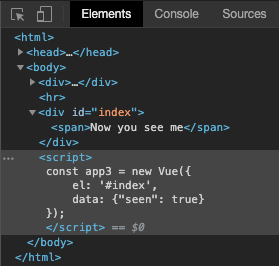
\includegraphics[width=6cm]{Rysunki/Rozdzial4/VueFlaskKod.png}
		\caption{Kod źródłowy strony wygenerowanej na podstawie listingu \ref{code:VueFlaskKod}. Przeglądarka \textit{Safari 13.1} pod systemy \textit{MacOS}.}	
		\label{fig:kodFlaskVue}
	\end{figure}
	

Jeżeli spojrzeć~w kod źródłowy strony~w przeglądarce wówczas można zauważyć, jak wyglądają już wygenerowane dane~z serwera dla podanego przykładu~i zauważyć, że metoda \textit{tojson} zwraca dane przesłane~w formie akceptowanej jako obiekt języka \textit{Javascript}, idealnie wpasowując się~w strukturę danych wymaganych przez pole \textit{data} obiektu instancji \textit{Vue}. Co sprawie, że można nimi operować bezpośrednio~w kodzie \textit{HTMLa} poprzez odpowiednie dyrektywy\cite{vuejs} (w tym przypadku dyrektywę \textit{v-if}) biblioteki \textit{Vue.js}.



W prosty sposób osiągnięto komunikację między serwerem, a biblioteką odpowiadającą za warstwę prezentacji. Niepotrzebne byłoby żadne dodatkowe narzędzie wystarczyło tylko wykorzystać elementy dostępne~w ramach obu tych frameworków.

Istnieją biblioteki pozwalające na szybkie tworzenie komponentów~w \textit{Vue}, nazywane \textit{UI Component Frameworks}. Są to zbiory gotowych elementów, do których wystarczy przekazać odpowiednio sformatowane dane~i ustawienia, a wygenerują one żądany fragment interfejsu użytkownika. W razie, gdy dostarczony komponent nie wygląda odpowiednio lub ma za mało funkcji to takie frameworki dostarczają proste \textit{API} do edycji ich wyglądu lub zastosowania, ale~w większości przypadków ich ustawienia~i dostępne możliwości są na tyle bogate, że ich większe zmiany są sporadyczne. Zastosowaną biblioteką~w projekcie jest \textit{ElementUI}\footnote{Link do dokumentacji \textit{ElementUI}: \url{https://element.eleme.io/}.}, można ją pobrać~z strony dokumentacji lub serwisu \textit{Github}\footnote{Link do repozytorium \textit{ElementUI} w serwisie \textit{github}: \url{https://github.com/ElemeFE/element}.} następnie przenieść do folderu \verb|static/js| i odpowiednio dodać do referencję~w pliku \textit{base.html} do:
 \begin{itemize}
  \item skryptu języka \textit{Javascript}: \verb|js/element-2.13.2/lib/index.js|
  \item arkuszy stylów biblioteki: \verb|js/element-2.13.2/lib/theme-chalk/index.css|
\end{itemize}

W folderze \textit{static/css} znajduje się plik \textit{main.css} odpowiada on za wszystkie style napisane~w projekcie monolitycznym~i podobnie do bibliotek~w języku \textit{Javascript} został on dołączony do pliku \textit{base.html}, więcej~o kaskadowych arkuszach stylów można przeczytać~w dokumentacji fundacji \textit{Mozilla}\cite{mdn}.

\chapter{Implementacja projektu - mikrousługi}
\label{roz5}
%=================================================================================================
W tym rozdziale opisany zostanie proces implementacji czterech mniejszych usług składających się~w jedną całą aplikację. Podstawową różnicą między tymi serwisami, a podejściem monolitycznym jest to, że każda~z nich działać będzie jako osobny serwer zajmując inny port. Zamiast porozumiewania się między komponentami przy pomocy struktury klas, będzie odbywać się to poprzez żądania \textit{HTTP} i stworzony~w celu interfejs \textit{API}.

\section{Zadania}
Pierwszą opisaną mikrousługą jest ta odpowiedzialna za zarządzanie zadaniami. Jest to osobna aplikacja napisana~w bibliotece \textit{Flask}. Podobnie jak~w przypadku usługi monolitycznej ma ona połączenie~z bazą danych przy pomocy \textit{ORMu}. Model zadania jest identycznie stworzony jak~w poprzednim projekcie. Korzystając~z biblioteki \textit{Flask-SQLAlchemy} tworzona jest instancja jej głównej klasy, do której przekazano obiekt \textit{app}, a następnie szablon klasy \textit{Task}. Różnicą jest to, że posiada ona metodę \textit{to\_dict}, której zadaniem jest zwracanie słownika~z wszystkimi polami, które będą dostępne dla klienta interfejsu \textit{API}. W związku~z tym, że wspomniany interfejs powinien być zgodny~z standardem \textit{JSON}, to nazwy kluczy~w słowniku są zapisane~w inny sposób niż standardowy dla języka \textit{Python}, a zgodny~z tym~w języku \textit{Javascript}\footnote{W języku \textit{Python} obwiązujący standard zapisywania nazw zmiennych to \textit{snake\_case}\cite{python}, gdzie poszczególne wyrazy odróżnia się poprzez podkreślnik. Natomiast~w języku \textit{Javascript} odbywa się to wyróżniając pierwszą literę drugiego słowa jako dużą. Konwencja ta nazwana jest \textit{camelCase}. Link do reszty informacji: \url{https://firefox-source-docs.mozilla.org/code-quality/coding-style/coding_style_js.html}.}. Pozwali to~w przyszłości na łatwiejsze operowanie danymi wewnątrz usługi odpowiedzialnej za interfejs użytkownika.

W związku~z tym, że każda~z poszczególnych aplikacji korzysta~z tej samej usługi bazodanowej ale innych baz, to należy~w pliku \textit{.env} dodać nową nazwę dla niej. Niestety nie zostanie ona stworzona automatycznie~i należy wykorzystać komendę \verb|psql -U postgres| i po uruchomieniu programu dodać nową bazę danych przy pomocy komendy \verb|CREATE DATEABASE postgrestasks;|. Takie rozwiązanie tworzy też kolejny problem, nie jest możliwe korzystanie~z relacji między poszczególnymi usługami. Zadania~i użytkownicy nie mogą być~z sobą powiązani przez klucz obcy. \textit{Flask-SQLAlchemy} udostępnia mechanizm \textit{binds}, który~w ramach zewnętrznego systemu pozwala tworzyć takie relacje\cite{flasksql}, ale odpowiednia implementacja tego mechanizmu jest dość trudna dla kilku mikrousług korzystających~z różnych baz danych. Struktura aplikacji tego nie wymaga, odpowiednio przygotowując funkcję odpowiedzialną za tworzenie zadań można przypisywać do nich \textit{identyfikator} użytkownika na podstawie przesłanych \textit{tokenów}. Zapewnią one integralność~i to, że te dane nie będą dostępne publicznie.

\begin{lstlisting}[language=Python, caption={Model zadania w mikrousłudze \textit{tasks} wraz z metodą \textit{to\_dict}.}]
class Task(db.Model):
    id = db.Column(db.Integer, primary_key=True)
    is_done = db.Column(db.Boolean)
    header = db.Column(db.String(68))
    body = db.Column(db.String(256))
    user_id = db.Column(db.Integer)
    timestamp = db.Column(db.DateTime, index=True, default=datetime.utcnow)

    def to_dict(self):
        return {
            'id': self.id,
            'isDone': self.is_done,
            'header': self.header,
            'body': self.body,
            'timestamp': self.timestamp
        }
\end{lstlisting}

Najważniejszą warstwą mikrousługi serwerowej jest \textit{API}. Odpowiadają za nie funkcje, które podobnie jak~w aplikacji monolitycznej otrzymują żądania~i odsyłają odpowiedzi. Nie są to natomiast odpowiedzi~w formie renderowanych szablonów, a obiektów typu \textit{JSON}. Biblioteka \textit{Flask} posiada metodę~o nazwie \textit{jsonify}, która pozwala~w łatwy sposób na przesyłanie odpowiedzi~w tej formie. Inną istotną sprawą jest utrzymanie spójnej struktury dla \textit{URLów} takich zapytań. W projekcie przyjęta będzie konwencja, gdzie żądany obiekt~w tym przypadku \textit{task} będzie przesyłany jako lista, gdy klient wyśle zapytanie \textit{GET} pod adres \verb|\tasks| (tu możliwe jest podanie parametrów zapytań do ich odfiltrowania). Dla metody {POST} z podanymi odpowiednimi danymi możliwe będzie stworzenie nowego celu, gdy potrzebne będzie poszczególne zadanie, wówczas wystarczy odpytanie adresu \verb|tasks/<int:id>|, gdzie \verb|<int:id>| odpowiada jego identyfikatorowi. Ten adres~w zależności od rodzaju zapytania będzie odpowiadać za usunięcie lub uaktualnienie podanego celu użytkownika.
W tej usłudze zapytanie kierowane na adres \verb|\|, \verb|\index| zwracać będzie wiadomość powitalną informującą~o rodzaju danych serwowanych przez aplikację. 
  
 \begin{lstlisting}[language=Python, caption={Funkcja \textit{index} zwracająca obiekt \textit{JSON}.}]
@app.route('/', method=['GET'])
@app.route('/index', method=['GET'])
def index():
    return jsonify(message="Welcome to task micro-service", success=True)
\end{lstlisting}

Nadal możliwe jest sprawdzenie zwróconych danych~w przeglądarce, wystarczy uruchomić aplikację~i~w pasu wyszukiwania wpisać \url{http://localhost:5000}, wówczas powinien zostać wyświetlony obiekt \textit{JSON}. Dla prostych zapytań typu \textit{GET} możliwe jest ich takie podejrzenie. Problemem jest przetestowanie innych metod \textit{HTTP}, ale istnieją do tego narzędzia takie jak prosty program konsolowy \textit{cURL} (\url{https://curl.haxx.se/}) lub okienkowa aplikacja \textit{Postman} (\url{https://www.postman.com/}).

\begin{lstlisting}[language=bash, caption={Testowe zapytanie wykonane przy pomocy programu \textit{cURL} w terminalu systemu \textit{Unix}.}]
$user@home: curl -i -H "Content-Type: application/json" http://localhost:5001/tasks

HTTP/1.0 200 OK
Content-Type: application/json
Content-Length: 59
Server: Werkzeug/1.0.1 Python/3.8.3
Date: Sun, 07 Jun 2020 19:58:18 GMT

{"message":"Welcome to task micro-service","success":true}
\end{lstlisting}

Każde zapytanie~o jakiekolwiek zadanie wymaga autentykacji (więcej~w rozdziale \ref{sec:autentykacja}) jest to warunek konieczny do jego otrzymania. Założenia aplikacji wykluczają możliwość podglądania zadań innych użytkowników, dlatego każda funkcja widoku najpierw sprawdza, czy obiekt \textit{request}\cite{flask} posiada nagłówek\cite{http} \textit{Authentication}, w którym jest token. Gdyby go nie było, to zwracana jest wiadomość~o braku autoryzacji, jeśli jest, to aplikacja kontaktuje się~z usługą odpowiedzialną za uwierzytelnianie~i pod adres \verb|/token-decode| wysyłany jest wspomniany wcześniej token. Następnie jeżeli wszystko jest~w porządku, to~w odpowiedzi usługa dostaje identyfikator użytkownika, który następnie jest wykorzystywany do tworzenia kwerend bazy danych. Dobrym przykładem może być widok odpowiedzialny za listowanie wszystkich zadań.

\begin{lstlisting}[language=Python, caption={Kod widoku odpowiedzialnego za listowanie zadań.}]
@app.route('/tasks', methods=['GET'])
def get_tasks():
    auth_header = request.headers.get('Authorization')
    user_id = auth_user(auth_header)
    if not isinstance(user_id, int):
        return jsonify(message='Authentication failed', success=False)

    tasks_list = Task.query.filter_by(user_id=user_id)
    return jsonify(tasks=[selected_task.to_dict() for selected_task in tasks_list], success=True)
\end{lstlisting}

Po otrzymaniu identyfikatora użytkownika sprawdzane jest, czy \textit{user\_id} jest typu numerycznego, tak aby upewnić się, czy to co zwróciła kontaktująca się~z serwisem od uwierzytelniania usługa jest informacją poprawną, którą można wykorzystać do wyszukiwania zadań. Korzystając~z mechanizmu kwerend biblioteki \textit{Flask-SQLAlchemy} wybierane są tylko cele należące do użytkownika wysyłającego zapytanie, a następnie przy pomocą mechanizmu przekształcania list (ang. \textit{list comprehension})\cite{python} wszystkie zadania są zamieniane na słowniki\footnote{Proces ten nazywany jest serializacją danych. W frameworkach takich jak \textit{Django} istnieją gotowe mechanizmy odpowiedzialne za ten mechanizm\cite{django}.}, umieszczane~w tablicy~i wysyłane przy pomocy funkcji \textit{jsonify}. Jest ona odpowiednikiem stworzenia nowego obiektu typu \textit{Request} do którego przekazany jest obiekt \textit{JSON}, stworzony przy wykorzystaniu standardowej biblioteki \textit{json} i metody \textit{dumps}\cite{flask}.

Poza funkcjami widoku, które wykorzystują metodę \textit{GET} są jeszcze adresy odpowiedzialne za tworzenie nowego zadania. Wówczas do parametru \textit{methods} przekazywana jest tablica~z ciągiem znaków, \textit{POST}. Wewnątrz tej funkcji poza sprawdzeniem poprawności tokenu, przeglądany jest obiekt \textit{request.json}, czy posiada on klucz \textit{header}, który jest jedynym wymaganym polem do utworzenia nowego zadania. Następnie otrzymane informacje są wykorzystane do utworzenia zadania, a jego dane są zwracane~w odpowiedzi.
\begin{lstlisting}[language=bash, caption={Testowe zapytanie \textit{POST} wykonane przy pomocy programu \textit{cURL} w terminalu systemu \textit{Unix}.}]
$user@home: curl -i -H "Content-Type: application/json" -H "Authorization: Bearer token_uzytkownika "  -X POST -d '{"header":"Read the docs"}' http://localhost:5001/tasks

HTTP/1.0 200 OK
Content-Type: application/json
Content-Length: 127
Server: Werkzeug/1.0.1 Python/3.8.3
Date: Sun, 07 Jun 2020 19:49:25 GMT

{"success":true,"task":{"body":"","header":"Read the docs","id":2,"isDone":false,"timestamp":"Sun, 07 Jun 2020 19:49:25 GMT"}}
\end{lstlisting}


W usłudze zaimplementowany jest również mechanizm aktualizacji celów, wówczas należy pod adres \verb|/tasks/<int:task_id>| wysłać żądanie \textit{PUT}. Cała procedura jest podobna jak ta do tworzenia nowego zadania, ale~w obiekcie \textit{request.json} sprawdzane jest, czy zostały przesłane wszystkie edytowalne pola wykorzystywane przy jego tworzeniu.

Ostatnim typem żądania jest usunięcie zadania, wówczas wykorzystywaną metodą jest \textit{DELETE}, a~w parametrze potrzebny jest jego number. Po uwierzytelnieniu, tworzona jest kwerenda, która odnajduje zadanie~o podanym identyfikatorze dla danej osoby. Możliwe jest to przy pomocy kwerendy \textit{AND}, którą łatwo implementuje się podając następne parametry funkcji \textit{filter\_by}. Po znalezieniu zadania wykorzystywana jest funkcja obiektu \textit{db.session} o nazwie \textit{delete}, a po zatwierdzeniu operacji wysyłana jest informacja~o usunięciu zadania wraz~z jego danymi.
\newpage
\begin{lstlisting}[language=Python, caption={Kod widoku odpowiedzialnego za usuwanie zadań.}]
@app.route('/tasks/<int:task_id>', methods=['DELETE'])
def delete_task(task_id):
	# czesc odpowiedzialna za uwierzytelnianie tokenu
	# ... 
    try:
        task_to_delete = Task.query.filter_by(
        		id=task_id,
         	user_id=user_id
        ).first()
        db.session.delete(task_to_delete)
        db.session.commit()
    except:
        return jsonify(
        		message="Cannot deleted task " + str(task_id),
        		sucess=False
        	)
    return jsonify(
    	message="Task deleted",
    	task=task_to_delete.to_dict(),
    	sucess=True
    )
 \end{lstlisting}
W razie jakichkolwiek błędów wszystkie wspomniane funkcję zwracają odpowiednie komunikaty wraz z informacją~o niepowodzeniu. Wykorzystując dekorator \textit{errorhandler} można również stworzyć odpowiedzi dla wszelkiego rodzaju błędów, których nie można obsłużyć wewnątrz zaimplementowanych widoków, takich jak skorzystanie~z nieistniejącego \textit{URLa} przez użytkownika\cite{flask}.

\begin{lstlisting}[language=Python, caption={Wykorzystanie dekoratora \textit{errorhander} do nadpisania kodu błędu \textit{404}.}]
@app.errorhandler(404)
def wrong_entrypoint(error):
    return jsonify(
    	error="API entrypoint not found",
    	success=False
    ), 404 
\end{lstlisting}

\section{Użytkownicy}
Kolejna potrzebną usługą jest ta odpowiedzialna za zarządzenie użytkownikami. Posiada ona także dostęp do bazy danych~z wykorzystaniem modułu \textit{Flask-SQLAlchemy}. Utworzone modele mają taką samą strukturę co~w aplikacji monolitycznej, jednak nie posiadają relacji~z zadaniami, ze względu na użycie wcześniej wspomnianego mechanizmów \textit{tokenów} nie ma potrzeby przechowywania żadnych relacji.

Głównym zadaniem tej mikrousługi jest tworzenie nowych użytkowników, zarządzenie ich logowaniem, wysyłaniem odpowiednich informacji~o nich. W tym celu zaimplementowano niżej określony schemat \textit{REST API}:
\begin{itemize}
  \item \verb|/|, \verb|/index| - zwraca metodą \textit{GET} informację, że podany \textit{URL} odnosi się do mikrousługi odpowiedzialnej za użytkowników.
  \item \verb|/users| - dla metody \textit{GET} jeżeli klient prześle poprawny \textit{token}, to zwraca informację takie jak email, nazwa użytkownika. Natomiast żądanie \textit{POST} tworzy nowego użytkownika~i zwraca dla niego \textit{token}, tak, aby mógł on mieć dzięki niemu dostęp do reszty funkcji aplikacji.
  \item \verb|/login| - wysyłając pod ten adres aplikacji żądanie \textit{POST} użytkownik może się zalogować. Po udanym procesie przesyłany jest nowy \textit{token} do uwierzytelniania.
  \item \verb|/logout| - pod tym adresem możliwe jest wylogowanie użytkownika, wówczas przesłany token wysyłany jest do usługi uwierzytelniającej~i tam dodawany do czarnej listy, tak aby nigdy więcej nie można było go użyć do korzystania~z funkcji dostępnych wyłącznie dla zalogowanej osoby.
\end{itemize}

Szczegółowa implementacja widoków jest podobna do tej~z usługi odpowiedzialnej za zadania. W każdym~z nich, gdzie wymagany jest \textit{token} najpierw sprawdzana jest jego poprawność, w razie braku,  zwracana jest odpowiednia wiadomość. Może zdarzyć się, że z jakiejś przyczyny token wygaśnie, wówczas aplikacja odpowiadająca za interfejs użytkownika automatycznie wyloguje go, tak aby użytkownik znów się zalogował przypisując mu nowo stworzony \textit{token}. Następnie na podstawie danych~z tokenu wybierany jest użytkownik~z bazy danych, a następnie odpowiednie dane są zwracane. Istnieją również adresy, gdzie przesyłane są dane~i sprawdzane jest, czy przyjęte do serwera żądanie posiada~w sobie wymagane informacje, w przeciwnym razie zwracana jest wiadomość~o błędzie. W funkcjach, gdzie tworzone są \textit{tokeny} przesyłane jest zapytanie do serwera tej usługi pod adres \verb|/token-encode| z identyfikatorem użytkownika jako parametrem. Wówczas tworzony jest ciąg binarny, kodowany później na klucz uwierzytelniający~i przesyłany jako odpowiedź serwera. Następnie~w odpowiednio sformatowanej informacji wysyłany jest on do klienta pod kluczem \textit{tokenAuth}.
Ostatnią istotną różnicą~w widokach jest wylogowywanie, metoda odpowiedzialna za nie jest podobnie zbudowana do \textit{get\_user} z tą różnicą, że adresem pod który serwer wysyła token to \verb|/token-blacklist|, który natomiast~w informacji zwrotnej potwierdza wylogowanie, gdy posiada ona status \textit{success} to przekazywane jest to klientowi, wówczas może on bezpiecznie usunąć nieaktualny token.

\section{Autentykacja}
\label{sec:autentykacja}
Autentykacja jest usługą pośrednią między listą zadań, a użytkownikami. Nie posiada ona otwartego portu\footnote{Wewnątrz kontenerów \textit{Dockera} można wskazać adres~z którego aplikacja będzie widoczna dla klienta\cite{docker}.}, aby była ona widoczna zewnątrz kontenera co sprawia, że kontakt~z nią jest jedynie możliwy wewnątrz wspólnego klastra kontenerów, stanowi to dodatkową warstwę zabezpieczeń. 

Inną istotną sprawą jest \textit{secret key}\cite{flask}, czyli ciąg znaków, który powinien być trzymany~w tajemnicy~i jest to ważny element tej usługi. Do generowania \textit{tokenów} wykorzystuje ona mechanizm \textit{JWT}\footnote{skrót od \textit{JSON Web Tokens}, jest to metoda uwierzytelniania wykorzystująca obiekty \textit{JSON} do bezpiecznej transmisji danych, więcej informacji~o \textit{JWT} można znaleźć na stronie: \url{https://jwt.io/introduction/}.}. Do szyfrowania informacji~i ich odszyfrowania korzysta się właśnie~z \textit{secret key}, to on stanowi gwarancję tego, że podane dane będą odszyfrowane~i zaszyfrowane pomyślnie. Wyciek wspomnianego ciągu znaków stanowi poważne zagrożenie dla poufności danych całego serwisu~i~w tym przypadku powinien on być natychmiastowo zastąpiony innym. Dla bezpieczeństwa takie klucze powinny być bardzo długą sekwencją losowych znaków\cite{flask}, których nie powinno się dać zapamietać\footnote{Więcej informacji~o generowaniu odpowiednich \textit{secret key} można znaleźć~w dokumentacji \textit{Flaska}\cite{flask}.}. Aplikacja wykorzystuje bibliotekę \textit{PyJWT}\footnote{Link do dokumentacji \textit{PyJWT}: \url{https://pyjwt.readthedocs.io/en/latest/}.} do tworzenia tokenów \textit{JWT}.


Widok odpowiedzialny za szyfrowanie kluczy ma adres \verb|/token_encode|, wewnątrz niego sprawdzane jest, czy otrzymał on żądanie~z identyfikatorem użytkownika (dzięki temu, że usługa dostępna jest wewnątrz kontenera, to niemożliwe jest przesłanie fałszywego identyfikatora~z zewnątrz), gdy metoda potwierdzi, że przyjęty format danych jest prawidłowy, to tworzony jest obiekt \textit{payload}. Zawiera on pola \textit{exp} z datą wygaśnięcia klucza, \textit{iat}, pole posiadające datę jego utworzenia~i \textit{user\_id}, identyfikator użytkownika\cite{Herman:2017}. Wszystkie te dane zostaną zaszyfrowane przy pomocy metody \textit{jwt.encode}, gdzie poza \textit{payload} przekazany jest również \textit{secret key} i rodzaj algorytmu wykorzystanego do zabezpieczenia danych. W tym przypadku jest to \textit{HS256}\footnote{Więcej~o algorytmach wykorzystywanych do szyfrowania \textit{tokenów} pod adresem: \url{https://jwt.io/}.}. Generuje on ciąg bajtów, których nie da się przesłać przez protokół \textit{HTTP}, dlatego przed wysłaniem powinno się na nim wywołać funkcję \textit{decode}.

Do odszyfrowania \textit{tokenu} wykorzystywany jest widok \verb|/token-decode|, otrzymuje on zaszyfrowany klucz~w obiekcie \textit{JSON}, następnie sprawdza, czy obiekt znajduje się~w bazie na czarnej liście (\textit{ang. blacklist}), jeśli nie, to jest odszyfrowywany przy pomocy metody \textit{jwt.decode}. Cała procedura zamknięta jest~w bloku \textit{try...except}, służy on do wyłapywania błędnych \textit{wyjątków}, a następnie~w kolejnym bloku są one odpowiednio obsługiwane\cite{python}. Aplikacja oczekuje błędu \textit{ExpiredSignatureError} i \textit{InvalidTokenError}, gdy jeden z nich wystąpi, to odsyłane są odpowiednie komunikaty~o błędzie, jeżeli nie, to odszyfrowane wiadomości~z tokenu są wysyłane~z powrotem.

Aplikacja posiada prosty model służący do przetrzymywania \textit{tokenów}, tak aby~w razie wylogowania użytkownika zachować ten klucz~w bazie~i~w razie potrzeby sprawdzić, czy nie został już wykorzystany. Klasa ta posiada takie pola jak \textit{id}, \textit{token}, który jest ciągiem znaków~o długości \textit{500} i \textit{blacklisted\_on}, które zachowuje informacje~o dacie, kiedy klucz został dodany do bazy danych. Wówczas klient wylogowując się przesyła obecny \textit{token} pod adres \verb|/token-blacklist|, gdzie następnie jest deszyfrowany, aby sprawdzić, czy dane~w nim są prawidłowe~i jeżeli są, to wtedy token zostaje zapisany, a usługa zarządzająca użytkownikami dostaje informacje~o pomyślnym zakończeniu procesu.

\section{Interfejs użytkownika}
\label{sec:ui}
W przypadku interfejsu użytkownika, będą to statyczne pliki serwowane przez \textit{Nginx}, ale~w celu rozwijania takich aplikacji powstały zestawy narzędzi, które to ułatwiają. Istnieją pakiety pozwalające na wygenerowanie skonfigurowanych projektów. W przypadku platformy \textit{Nuxt.js}, czyli biblioteki do statycznego renderowania stron~w \textit{Vue.js} jest to \textit{nuxt-create-app}\cite{nuxtjs}. Z pomocą tej aplikacji została stworzona stosowna struktura projektu~i wybrany zestaw programów wykorzystywanych~w ramach niego, takich jak odpowiedni preprocesor do plików \textit{CSS}, biblioteka \textit{ElementUI}. W celu zapewnienia dodatkowych opcji doinstalowano przy pomocy narzędzia \textit{Yarn}\footnote{Link do dokumentacji narzędzia \textit{Yarn}: \url{https://yarnpkg.com}.} takie moduły jak \textit{@nuxt/http} i \textit{@nuxtjs/proxy}. Nazwy tych narzędzi należało podać~w pliku \textit{nuxt.config.js} w sekcji \textit{modules}. Moduł \textit{Proxy} pozwala na skonfigurowanie~w tym samym pliku, gdzie jest informacja~o jego wykorzystaniu, poprzez dodanie obiektu \textit{proxy}, prostego przekierowania adresów, wówczas gdy zostanie odpytany serwer developerski~o \textit{URL} podany~w konfiguracji, to automatycznie przekieruje on żądanie do jednej~z aplikacji \textit{Flaska}.
\begin{lstlisting}[language=Javascript, caption={Fragment pliku \textit{nuxt.config.js} z konfiguracją obiektu \textit{proxy}.}]
  /*
  ** Nuxt.js modules
  */
  modules: [
    '@nuxt/http',
    '@nuxtjs/proxy',
  ],
  proxy: {
    '/tasks-api': {
      target: 'http://tasks:5000/',
      pathRewrite: {
        '^/tasks-api': '/'
      },
    },
    '/users-api': {
      target: 'http://users:5000/',
      pathRewrite: {
        '^/tasks-users' : '/'
      }
    },
  },
\end{lstlisting}

\textit{Nuxt.js} wykorzystuje mechanizm renderowania plików po stronie serwera (ang. \textit{Server Side Rendering}), co~w rezultacie odpowiada za to, że każda ścieżka~w aplikacji będzie oddzielnym plikiem \textit{HTML}\cite{nuxtjs}. Pliki odpowiedzialne za generowanie takich ścieżek są~w projekcie umiejscowione~w katalogu \verb|pages/|. W przypadku list zadań potrzebne jest jednak dynamiczne generowanie adresów. \textit{Nuxt.js} również posiada taki mechanizm\cite{nuxtjs}. Wówczas należy stworzyć wewnątrz omówionego folderu kolejny~o nazwie odpowiadającej pożądanej ścieżce~i wewnątrz umieścić plik \textit{index.html}, to on będzie renderowany, gdy użytkownik poda~w pasku przeglądarki \verb|/tasks/| (dla listy zdań). Gdy będzie potrzebował celu~o określony identyfikatorze, wtedy należy utworzyć wewnątrz tego folderu plik~o nazwie \textit{\_id.vue}. Taką strukturę~w nazwie aplikacja \textit{Nuxt.js} identyfikuje jako szablon, który należy wczytać przy podaniu adresu \verb|/tasks/1|. Argument przekazany w adresie \textit{URL} framework rzutuje na zmienną o nazwie \textit{id} we wczytanym pliku \textit{HTML}\cite{nuxtjs}.

Do zarządzania ścieżkami, aby nie były one dostępne dla niezalogowanego użytkownika wykorzystano mechanizm \textit{middleware}\cite{nuxtjs}. Jest to zestaw funkcji, które można bezpośrednio wywołać przed przejściem użytkownika na inny adres. Wewnątrz nich sprawdzane będzie, czy klient ma zapisany~w globalnej zmiennej przeglądarki \textit{localStorage}, która przechowuje informacje~z danej witryny aż do zamknięcia sesji przeglądarki\cite{mdn}, \textit{token}, jeżeli tak to korzystając modułu~z \textit{@nuxt/http} do argumentu obiektu globalnego aplikacji \textit{Nuxt.js}, \textit{\$http} jest on dołączany przy pomocy metody \textit{setToken}.

Po dodaniu do nagłówka sekcji uwierzytelnienia możliwe jest pobieranie danych~z zabezpieczonych adresów aplikacji serwerowej. W przypadku braku możliwości pozyskania tokenów lub, gdy serwer zwróci błąd przy jego odszyfrowaniu, to przy wykorzystaniu argumentu funkcji \textit{middleware}, \textit{context} i metody \textit{redirect} należy użytkownika przekierować do strony logowania, tak aby zalogował się on jeszcze raz~i pobrał nowy \textit{token}.

Biblioteka \textit{@nuxt/http} pozwala~w prosty sposób na pobieranie~i wysyłanie żądań do aplikacji serwerowych, korzystając~z funkcji \textit{fetch} wewnątrz komponentu\cite{nuxtjs}. Posiada ona również zestaw metod, dzięki którym można sprawdzić stan zapytania~i~w zależności od jego wyniku wysłać odpowiednie komunikaty.

\begin{lstlisting}[language=Javascript, caption={Przykład komponentu wczytującego listę zadań.}]
<template>
  <div>
   	<p v-if="$fetchState.pending">Fetching posts...</p>
   	<p v-else-if="$fetchState.error">
   		Error while fetching posts: {{ $fetchState.error.message }}
   	</p>
    <ul v-else>
       <li v-for="task of tasks" :key="task.id">
       	<n-link :to="`/tasks/${task.id}`">
       		{{ task.header }} {{ task.body }} {{ task.isDone }} </n-link>
       </li>
   </ul>
  </div>
</template>
<script>
//...
export default {
  data () {
    return {
      tasks: []
    }
  },
  async fetch () {
    const request = await this.$http.$get('tasks-api/tasks')
    if (request.success) {
      this.tasks = request.tasks
    }
  }
}
</script>
\end{lstlisting}

Wykorzystanie prostego serwera \textit{proxy} sprawiło, że nie jest potrzebne podawanie całego adresu, a wystarczy jedynie, aby aplikacja wysłała żądanie pod odpowiedni \textit{URL} w swojej domenie. Mechanizm odpowiedzialny za przekierowywanie wyśle to zapytanie do jednej~z aplikacji serwerowych.
\chapter{Konteneryzacja}
\label{roz6}
%=================================================================================================
Konteneryzacja aplikacji przy pomocy platformy \textit{Docker} zapewnia działanie systemu niezależnie od sprzętu programisty\cite{Ziade:2018}, ale również może być wykorzystana do stworzenia środowiska produkcyjnego\cite{Ziade:2018} i integracji~z wybraną infrastrukturą serwerową. Serwisy takie jak \textit{Amazon Web Services} posiadają gotowe rozwiązania do publikacji aplikacji wewnątrz kontenerów\cite{aws}.

 W tym rozdziale przedstawione zostanie przygotowanie konfiguracji środowiska rozwojowego (deweloperskiego) i produkcyjnego przy wykorzystaniu narzędzi \textit{Docker}, \textit{Docker Compose}, aplikacji \textit{Gunicorn} i \textit{Nginx}\cite{Herman:2020}.
 
 Fundamentem działania platformy są kontenery, czyli procesy systemu \textit{Linux} z dodatkowymi funkcjami pozwalającymi na ich izolację od maszyny użytkownika. Jednym~z aspektów, który pozwala na odseparowanie każdego~z kontenerów jest to, że posiadają one własny system plików dostarczany przez \textbf{obrazy Dockera} (ang. \textit{docker images}), które mają~w sobie wszystkie potrzebne zależności, pliki binarne~i kody źródłowe\cite{docker}. Ich ważną właściwością jest to, że łatwo możne je przenosić, dzięki czemu twórcy platformy \textit{Docker} stworzyli serwis \textit{Docker Hub} w którym są one przechowywane\cite{docker}. Każdy użytkownik może stworzyć własny obraz, a następnie go udostępnić innym, tak, aby bez problemu można było go wykorzystać~w tworzonej aplikacji. W efekcie każdy język programowania, wiele bibliotek~i narzędzi posiada swoje odpowiedniki~w formie obrazów \textit{Dockera}. Nie jest potrzebne instalowanie interpretera języka \textit{Python}, wystarczy, że zastanie pobrany odpowiedni obraz, z którego będzie można korzystać jak~z normalnie zainstalowanej wersji na fizycznej maszynie.
 
\begin{lstlisting}[language=Bash, caption={Proces pobrania i wykorzystanie przykładowego obrazu \textit{Dockera}.}, label={code:docker}]
$user@home: docker run  python:3.8.3-buster
Unable to find image 'python:3.8.3-buster' locally
3.8.3-buster: Pulling from library/python
Status: Downloaded newer image for python:3.8.3-buster
$user@home: docker image ls
python              3.8.3-buster        659f826fabf4        3 weeks ago         934MB
$user@home: docker run --name python -it python:3.8.3-buster
Python 3.8.3 (default, May 16 2020, 07:08:28)
[GCC 8.3.0] on linux
Type "help", "copyright", "credits" or "license" for more information.
>>>
\end{lstlisting}

Każdy obraz, przechowywany na platformie \textit{Docker Hub}, poza nazwą posiada jeszcze, po dwukropku, numer wersji, a także, po myślniku, nazwę systemu, który został wykorzystany przy konteneryzacji. W przypadku listingu \ref{code:docker} jest to dystrybucji systemu \textit{Debian} o nazwie \textit{Buster}\footnote{Informację o wersjach systemu operacyjnego \textit{Debian} można znaleźć pod adresem: \url{https://www.debian.org/releases/}.}.

Aplikacja \textit{Docker} może automatycznie tworzyć obrazy odczytując instrukcję~z pliku \textit{Dockerfile}. Jest to dokument tekstowy wykorzystujący specjalną składnie, dzięki której można zarządzać systemem znajdującym się wewnątrz kontenera, tak aby odtworzył on wymagane środowisko. W projekcie serwisu monolitycznego znajdują się dwa takie pliki pozwalające na zbudowanie obrazu, który uruchomi aplikację opartą~o bibliotekę \textit{Flask}. Pierwszy odpowiada za przygotowanie środowiska deweloperskiego, drugi produkcyjnego. \textit{Flask} posiada wbudowany serwer (\textit{flask run}), ale nie jest on przystosowany do bycia efektywnym, stabilnym~i bezpiecznym\cite{flask}. Wiele bibliotek ma podobne problemy~i także oferuje inne narzędzia do obsługi zapytań~w konfiguracji produkcyjnej\cite{django}. Aplikacje uruchomione przy wykorzystaniu narzędzi dostarczonych przez platformę są przystosowane do rozwijania, przekazywania błędów programiście~i prostego debugowania, ale nie są one zalecane do wykorzystania przy wdrożeniu, dlatego potrzebne są przynajmniej dwa pliki \textit{Dockerfile}.

Pierwszy~z nich odpowiedzialny jest za środowisko deweloperskie. Najpierw pobiera on obraz \verb|python:3.8-alpine|, a następnie ustanawia obecny katalog jako \verb|/code|. Następnie kopiuje plik \textit{requirements.txt}, umieszczone są~w nim wszystkie wymagane biblioteki wraz~z ich wersjami. Kolejną czynnością jest zainstalowanie wymaganych przez system \textit{Linux} paczek, tak aby móc później zbudować potrzebne biblioteki języka \textit{Python}. Na końcu kopiowana jest zawartość całego folderu~w którym znajduje się plik \textit{Dockerfile} do systemu plików kontenera~i wcześniej ustawionego folderu \textit{WORKDIR}.

\begin{lstlisting}[language=Bash, caption={Plik \textit{Dockerfile} wykorzystany do zbudowania obrazu aplikacji monolitycznej.}, label={code:dockerfile}]
FROM python:3.8-alpine

WORKDIR /code

COPY requirements.txt .

RUN \
 apk add --no-cache postgresql-libs && \
 apk add --no-cache --virtual .build-deps gcc musl-dev postgresql-dev && \
 python3 -m pip install -r requirements.txt --no-cache-dir && \
 apk --purge del .build-deps

COPY . .
\end{lstlisting}

\textit{Dockerfile} z listingu \ref{code:dockerfile} działa dla wszystkich aplikacji napisanych~w \textit{Flasku}, czyli również tych stworzonych na potrzeby rozwiązań mikrousługowych. Należało utworzyć je osobno dla każdej~z usług.

Uruchamianie osobno kilku kontenerów, które~z sobą współpracują może być uciążliwe, a dodatkowo wymaga wpisywania wszystkich parametrów~w linii poleceń, dlatego twórcy platformy \textit{Docker} przygotowali narzędzie \textit{Docker Compose}. Pozwala ono na definiowanie~i uruchamianie kilku kontenerowych aplikacji, którymi można zarządzać poprzez odpowiednią konfigurację plików~o formacie \textit{YAML}, a następnie przy pomocy jednej komendy włączać wszystkie serwisy\cite{docker}. Będą one wówczas działać~w odizolowanym środowisku, wewnątrz którego kontenery mogą się między sobą porozumiewać\cite{docker}.

Atutem takiego rozwiązania jest uproszczona integracja usługi bazodanowej~z resztą aplikacji. Wystarczy stworzyć prosty serwis~i podać odpowiedni obraz, a następnie udostępnić port, który zostanie wykorzystany do łączenia się między kontenerami. Niestety nie jest możliwe ustalenie, która usługa powinna uruchomić się najpierw, co~w rezultacie sprawia, że baza danych może być niedostępna przez pierwsze kilka sekund po starcie serwisu webowego. Nie jest to wadą tego rozwiązania, ale warto~o tym pamiętać. Istniej parę skryptów dostępnych~w serwisie \textit{Github}, które sprawiają, że można ten błąd naprawić, jeden~z nich został wykorzystany przy implementacji środowiska produkcyjnego\footnote{Wspomniany skrypt został udostępniony~w artykule \cite{Herman:2020} na podstawie, którego została przygotowana konfiguracja produkcyjna.}.

\begin{lstlisting}[language=Bash, caption={Plik \textit{docker-compose.yml} wykorzystany do uruchomienia aplikacji monolitycznej.}, label={code:dockercompose}]
version: '3'
services:
  db:
    image: postgres:12
    env_file: .env
    volumes:
      - .pgdata:/var/lib/postgresql/data

  web:
    env_file: .env
    build: .
    depends_on:
      - db
    command: python -m flask run --host 0.0.0.0
    ports:
      - "5000:5000"
    volumes:
      - ./mono:/code/mono
      - ./bin:/code/bin
      - ./.env:/code/.env
      - ./main.py:/code/main.py
      - ./config.py:/code/config.py
      - ./migrations:/code/migrations
\end{lstlisting}

Każda konfiguracja \textit{Docker Compose} wymaga podania numeru wersji, tak aby program mógł odpowiednio rozpoznać strukturę pliku. Następnie wyróżniona jest specyfikacja dla serwisów (można też skonfigurować sieci lub wolumeny\cite{docker}), ich nazwa, a później poszczególne właściwości, takie jak pliki konfiguracyjne~z których mają korzystać, miejsce gdzie znajduje się \textit{Dockerfile} (klucz \textit{build}), komenda uruchamiająca aplikację, porty, które mają zostać udostępnione. Na końcu mapowany jest system plików, tak aby byłby one dostępne wewnątrz kontenera~i narzędzie mogło~z nich skorzystać~w celu uruchomienia aplikacji.

Podany \verb|env_file|, to plik tekstowy przechowujący zmienne systemu \textit{Linux}\cite{docker}, takie jak \textit{secret key} aplikacji, dane~o nazwie, użytkowniku~i haśle do bazy danych, dlatego nie powinien on być dostępny publicznie, w szczególności zapisywany~w repozytorium. Zwyczajem jest tworzenie szablonu takiego pliku, tak aby programista mógł go skopiować, a następnie tylko wypełnić odpowiednimi informacjami. 

W przypadku aplikacji opartej~o mikroserwisy, plik~z listingu \ref{code:dockercompose} posiada zamiast jednego serwisu \textit{web} trzy: \textit{users}, \textit{tasks}, \textit{tokens} o bardzo podobnej konfiguracji, z tą różnicą, że wartości portów muszą być dla nich inne, tak, aby dwie aplikacje nie działały na jednym. Usługa \textit{tokens} w ogóle nie udostępnia portu\footnote{Zgodnie~z założeniami usługi do uwierzytelniania (rozdz. \ref{sec:autentykacja}) nie może być ona dostępna zewnątrz klastra kontenerów.}.

Innym istotnym faktem, jest to, że aplikacje napisane~w bibliotece \textit{Flask}, aby były dostępne zewnątrz kontenera muszą być uruchomione na hoście \verb|0.0.0.0|, jest to konwencja pozwalająca na przekazanie systemowi operacyjnemu, aby nasłuchiwał żądań serwera dla wszystkich publicznych adresów \textit{IP}\cite{flask}. Sprawia to, że można się~z aplikacją połączyć~w ramach fizycznej maszyny, na której działa, wykorzystując na przykład przeglądarkę~i wpisując~w niej adres \url{http://localhost:5000}.

Do uruchomienia aplikacji~z wykorzystaniem narzędzia \textit{Docker Compose} należy~w folderze, gdzie znajduje się plik~z konfiguracją wpisać~w terminalu \verb|docker-compose up|, wówczas wszystkie kontenery najpierw się zbudują, a następnie uruchomią. Proces budowy można wymusić przy pomocy komendy \verb|docker-compose build|. W celu wyłączenia kontenerów można spróbować przerwać proces wciskając kombinację klawiszy \textit{control+c}, gdy to się nie powiedzie, to należy wpisać komendę \\ \verb|docker-compose down| i poczekać na informację~o zakończeniu ich działania\cite{docker}.

W aplikacji opartej~o mikrousługi jest jeszcze konfiguracja serwisu odpowiedzialnego za dostarczenie interfejsu użytkownika. Wykorzystuje ona obraz \\ \verb|node:14.1.0-strech| w którym zainstalowane jest narzędzie \textit{Yarn} (jego opis znajduje się~w rozdziale \ref{sec:ui}), które instaluje wszystkie wymagane moduły~w folderze \verb|/tmp/node_modules|, a następnie kopiuje je do projektu~w systemie plików kontenera. W pliku \textit{docker-compose.yml} serwis nazywa się \textit{frontend} i jest uruchamiany komendą \verb|yarn dev|. Ma on ustawione przekierowanie na porty \textit{8000:8000} i również~w tym przypadku należy ustawić zmienną host na \verb|0.0.0.0|, aby kontener był dostępny~z zewnątrz. Zmiana tej właściwości nie jest możliwa poprzez konfiguracje \\ \textit{docker-compose.yml} ale dodanie odpowiedniej opcji~w pliku \textit{nuxt.config.js}\cite{nuxtjs}.

Konfiguracja produkcyjna przechowywana jest~w oddzielnych plikach \textit{Dockerfile.prod} i \textit{docker-compose.prod.yml}. W przypadku aplikacji opartych~o bibliotekę \textit{Flask}. Proces budowy obrazu posiada dwie fazy\cite{Herman:2020}. Pierwsza ma za zadanie zbudowanie jej do pakietu \textit{wheel} przy pomocy komendy \verb|pip wheel|. W drugiej natomiast pakiet ten jest instalowany, a następnie serwowany przy pomocy aplikacji \textit{Gunicorn}, która odpowiada za obsługę żądań. W przypadku plików statycznych są one dzielone między serwisy \textit{web}, a \textit{nginx} przy wykorzystaniu wspólnych \textit{wolumenów}\cite{docker}. Tworzone są one~z użyciem \textit{Dockerfile}'a~w katalogu \verb|./nginx|, wewnątrz którego usuwany jest domyślny plik~z ustawieniami (\textit{default.conf}), a kopiowany jest ten~z dysku maszyny fizycznej(\textit{nginx.conf}). W nim również znajduje się konfiguracja \textit{load balancera}\cite{nginx}. Ustawiony jest serwer nadrzędny (ang. \textit{upstream}), który wykorzystuje aplikację \textit{Gunicorn}, a następnie~w sekcji serwer podawana jest jego lokalizacja jako \textit{proxy\_pass}, dzięki czemu każde zapytanie jest odpowiednio do niego przydzielane. Ostatnią czynnością jest podanie ścieżki do plików statycznych, tak aby były one dostępne dla serwisu pod adresem \verb|/static/|. W przypadku aplikacji opartej~o mikrousługi podane są dwa serwery nadrzędne, a lokalizacja \verb|\| odpowiada ścieżce do zbudowanych\footnote{W celu zbudowania projektu wykorzystano komendę \textit{yarn generate}, która tworzy aplikację jako strukturę statycznych plików \textit{HTML} w katalogu \textit{dist}.} plików projektu \textit{Nuxt.js}\cite{nuxtjs}. W tym miejscu zamiast serwera \textit{proxy} wykorzystana jest opcja \textit{try\_files}\cite{nginx}. Po zakończeniu konfiguracji wszystkie włączone usługi powinny być dostępne pod jednym adresem \verb|http://localhost:80/|. Podczas uruchamiania narzędzia \textit{Docker Compose} należy pamiętać~o wpisaniu polecanie uwzględniającego konfigurację produkcyjną: \verb|docker-compose -f docker-compose.prod.yml up|.

W przypadku integracji~z dowolna platformą dostawcy usług internetowych wystarczy, że będzie ona posiadać zainstalowaną usługę \textit{Docker} (lub będzie można ją doinstalować), następnie wystarczy zmodyfikować konfigurację serwera, tak, aby przekierowała ona wszystkie połączenia do serwera nadrzędnego, który będzie ustawiony pod adresem \verb|http://localhost:80/|. Dla platformy \textit{AWS} jest to odpowiednie nadpisanie zmiennych globalnych narzędzia \textit{Amazon Elastic Container Service}\cite{aws}. Natomiast~w przypadku prywatnych wirtualnych serwerów \textit{VPS} należy zainstalować na nich usługę \textit{Nginx} i~w podobny sposób jak przy konfiguracji kontenera dodać serwer nadrzędny~i wykorzystać opcję \textit{proxy\_pass} do przekierowania żądań do aplikacji~w kontenerze\footnote{Link do artykuły wyjaśniającego konfigurację na platformie \textit{DigitalOcean}: \url{https://www.digitalocean.com/community/tutorials/docker-explained-how-to-containerize-and-use-nginx-as-a-proxy} (autor: O.S Tezer, data publikacji: 16.12.2013).}.

\chapter{Porównanie i analiza aplikacji}
\label{roz7}
%=================================================================================================
Poprzednie rozdziały przedstawiły proces tworzenia~i wdrażania aplikacji monolitycznej, a także jej odpowiednika opartego~o mikrousługi. Po opracowaniu środowiska produkcyjnego możliwe jest przeprowadzenie badań mających na celu porównanie obu tych systemów. Istotne~w nich będą takie parametry jak wydajność, skalowalność~i łatwość implementacji.

\section{Cel~i zakres badań}
Celem badań jest przeprowadzenie porównania wydajności obu serwisów~w środowiskach produkcyjnych. Przebadane zostanie to jak podział aplikacji na mniejsze usługi wpływa na ogólną sprawność serwisu~w porównaniu do jednej scentralizowanej aplikacji. Następnie sprawdzone zostanie, jak zmieniają się osiągi aplikacji przy ich skalowaniu, czyli zwiększaniu ilości zasobów sprzętowych~i liczby kontenerów, które mogą obsługiwać żądania. Analizie zostanie poddana implementacja poszczególnych serwisów, tak, aby porównać otrzymane wyniki do zastosowanych technologii, skali projektu, trudności~w przygotowaniu architektury~i zastosowania danych rozwiązań technologicznych. Celem badań jest wskazanie podobieństw~i właściwości poszczególnych podejść. Znalezienie ich atutów~i wad, a następnie wskazanie przypadków, gdzie wykorzystanie danej architektury byłoby korzystniejsze.

Do testów wydajności wykorzystane będzie narzędzie \textit{Boom}. Jest to biblioteka napisana~w języku Python przez autora książki \textit{Rozwijanie mikrousług~w Pythonie}\cite{Ziade:2018}, której zadaniem jest przeprowadzenie testów obciążeniowych serwera. Przesyła ona do niego zadaną ilość żądań symulując ruch~w danym serwisie, a następnie dla każdego~z nich mierzy czas. Wyniki tych operacji uśrednia podając całkowity czas przeprowadzonego testu, najszybciej~i najdłużej wykonane żądanie, a także ich średni czas, amplitudę, ilość żądań na sekundę.
\newpage
\begin{lstlisting}[language=Bash, caption={Przykładowy test przy wykorzystaniu narzędzia \textit{Boom}.}]
$user@home: boom http://localhost:80 -c 10 -n 100
Server Software: nginx/1.17.10
Running GET http://127.0.0.1:80
	Host: localhost
Running 100 queries - concurrency 10
[=================================================================>] 100% Done

-------- Results --------
Successful calls		100
Total time        		0.8767 s
Average           		0.0839 s
Fastest           		0.0317 s
Slowest           		0.1165 s
Amplitude         		0.0848 s
Standard deviation		0.016234
RPS               		114
BSI              		Pretty good

-------- Status codes --------
Code 200          		100 times.

-------- Legend --------
RPS: Request Per Second
BSI: Boom Speed Index
\end{lstlisting}

Natomiast do przeprowadzenia analizy skalowalności również zostanie wykorzystane narzędzie \textit{Boom}, aby porównać jak zwiększenie ilości serwisów wpływa na wydajność aplikacji. Samo skalowanie aplikacji może zostać przeprowadzone przy wykorzystaniu platformy \textit{Docker}, posiada ona funkcję zwiększenia ilości zasobów takich jak ilość rdzeni, pamięci \textit{RAM}. Proces zmiany tych wartości nazywany jest \textit{skalowaniem~w pionie}\cite{Folwer:2019}.

Do \textit{skalowania~w poziomie}\cite{Folwer:2019} zostanie wykorzystana możliwość zwiększenia ilości kontenerów dla danego serwisu~w ramach narzędzia \textit{Docker Compose}. Przy pomocy polecenia \verb|docker-compose up --scale nazwa_serwisu=ilosc_kontenerow|, można przypisać ile kontenerów powinna mieć dana usługa~i dzięki temu zwiększyć przepustowość żądań aplikacji\cite{docker}.

W celach sprawdzenia łatwości implementacji danego rozwiązania przeprowadzone zostanie analiza poszczególnych fragmentów obu serwisów, ich rozbudowania, wymaganych zależności~i ocena zastosowanych rozwiązań architektonicznych.

\section{Wydajność}
W każdym badaniu przeprowadzonym przy pomocy programu \textit{Boom} wykorzystano takie same parametry, symulując ruch dla \textit{100} użytkowników, którzy wysyłają maksymalnie \textit{1000} żądań. Na początku przeprowadzono pomiar dla wszystkich dostępnych adresów~w obu serwisach. Aplikacja monolityczna obsługuje informację~o użytkowniku korzystając~z zmiennych globalnych, które są dostępne~w każdym~z widoków, dlatego nie potrzebuje ona zwracać informacji~o nim, w przeciwieństwie do aplikacji opartej~o mikrousługi, która na wykresie \ref{fig:microczasy} będzie miała, z tego powodu, jeden adres więcej. Dla zapytania \verb|\index| wyróżniono jeszcze przypadek, gdy użytkownik jest zalogowany (\textit{logged}). Wyniki przedstawiono na poniżej wykresach:
\begin{figure}[h!]
	\centering
		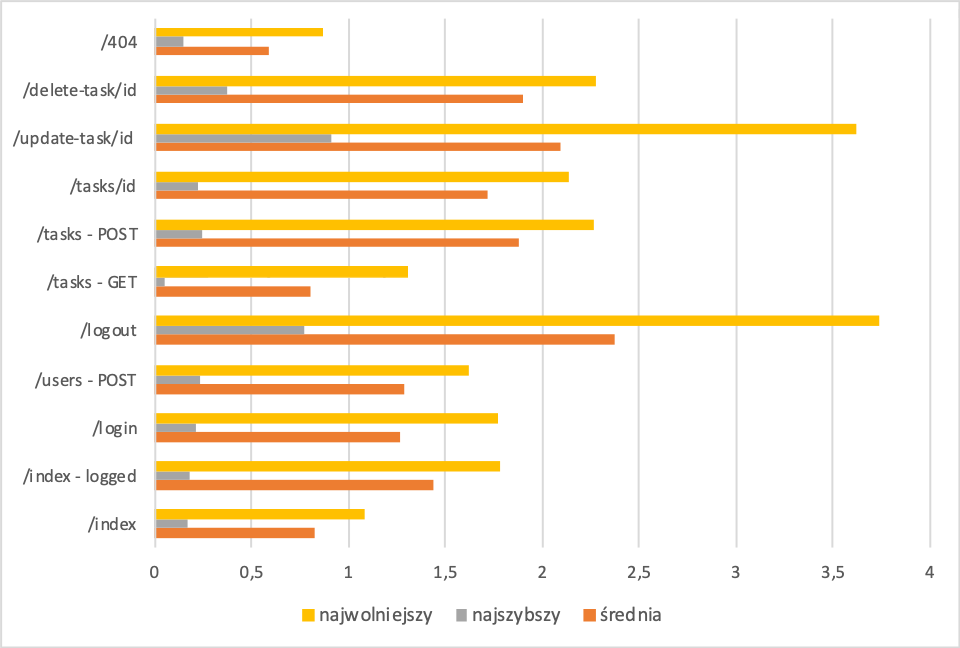
\includegraphics[width=12cm]{Rysunki/Rozdzial7/mono-zad.png}
		\caption{Czasy żądań (ms) dla każdego z adresu w aplikacji monolitycznej.}
		\label{fig:monoczasy}
	\end{figure}
\begin{figure}[h!]
	\centering
		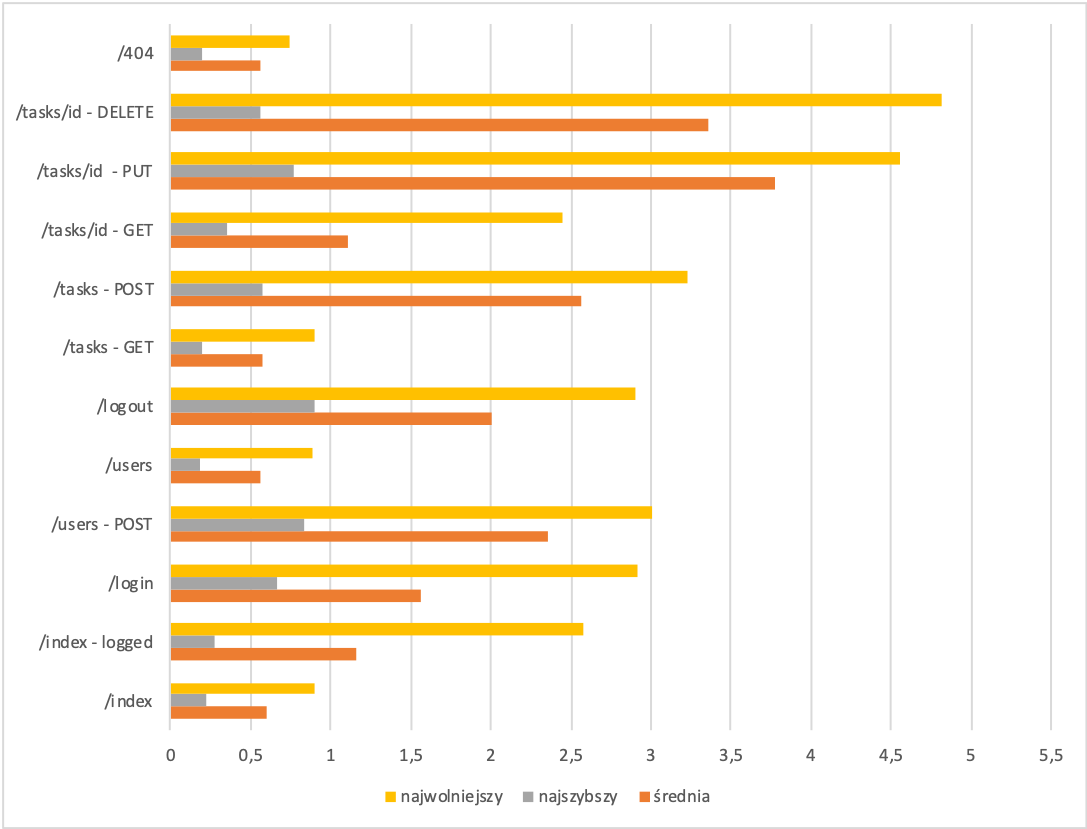
\includegraphics[width=12cm]{Rysunki/Rozdzial7/micro-zad.png}
		\caption{Czasy żądania (ms) dla każdego z adresu w aplikacji mikrousługowej.}
		\label{fig:microczasy}
	\end{figure}

Z wykresów (\ref{fig:microczasy}, \ref{fig:monoczasy}) wynika, że dla prostszych informacji do zwrócenia takich jak te~z adresów: \textit{index}, strona \textit{404}, obie aplikacje mają podobne wyniki~i zabierają im one najmniej czasu. Więcej zajmuje natomiast zwrócenie stron przy użyciu zapytania \textit{GET}, w tym przypadku widać, że nie ma reguły~i średni czas dla nich jest różny. Najdłużej~w aplikacji monolitycznej wykonywane są żądania odpowiadające za wylogowanie użytkownika, a także aktualizację zadania. Z kolei~w serwisie opartym~o mikrousługi najdłuższe jest usunięcie, a także jak~w przypadku pierwszej aplikacji zaktualizowanie zadania użytkownika.  Wynikać to może~z tego, że te żądania wymagają zweryfikowania wszystkich danych przesłanych~w zapytaniu, a następnie nadpisania lub usunięcia danego obiektu~z bazy danych.

Aplikacja oparta~o mikrousługi ma ogólnie gorsze średnie czasy~i dłuższe odpowiedzi, mimo, że dane zwracane przez serwer to proste obiekty \textit{JSON}, a nie całe struktury \textit{HTML} jak~w serwisie monolitycznym. Widocznie, przy niewielkich rozmiarach serwisów rodzaj przesyłanych danych nie wpływa na szybkość działania usług, a może go mieć ich \textit{serializacja} (mikrousługi) do formatu \textit{JSON}.

\section{Skalowalność}
W panelu ustawień platformy \textit{Docker} są funkcje odpowiedzialne za zarządzanie zasobami. Wśród nich możliwość zmiany ilości rdzeni procesora~i \textit{RAMu}, sterując tymi zależnościami zbadany będzie ich wpływ na szybkość zapytań.

\begin{figure}[h!]
	\centering
		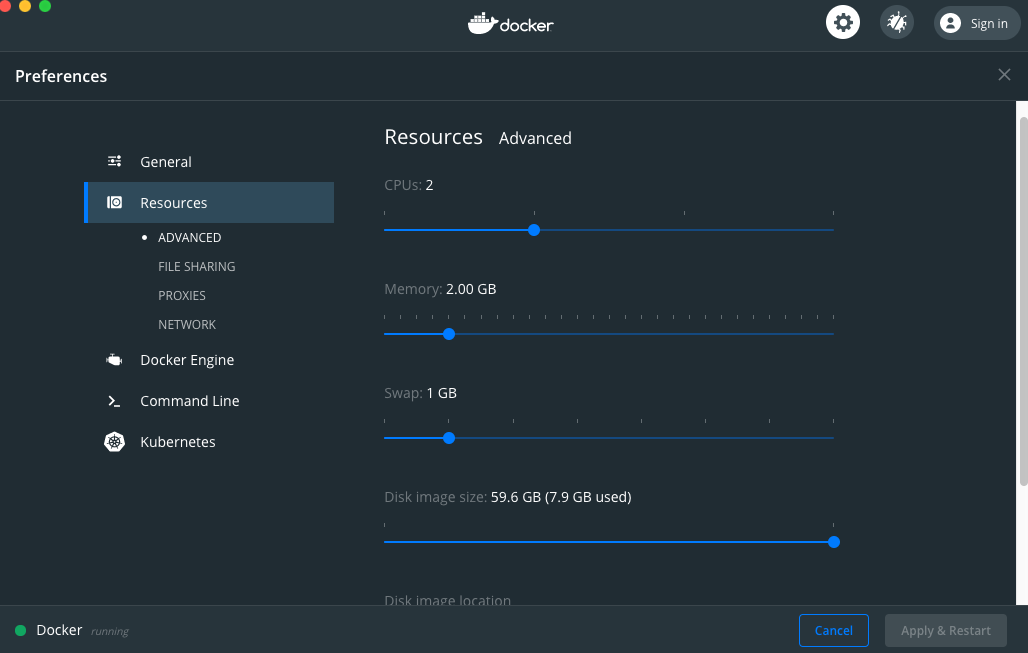
\includegraphics[width=12cm]{Rysunki/Rozdzial7/dockerpanel.png}
		\caption{Zakładka do zarządzania zasobami w ustawieniach platformy \textit{Docker}.}
		\label{fig:microczasy}
	\end{figure}
Badania obejmą sprawdzenie zmiany szybkości odpowiedzi serwera~w zależności od zasobów. Do ich przeprowadzania również wykorzystano narzędzie \textit{Boom}.

\begin{figure}[h!]
	\centering
		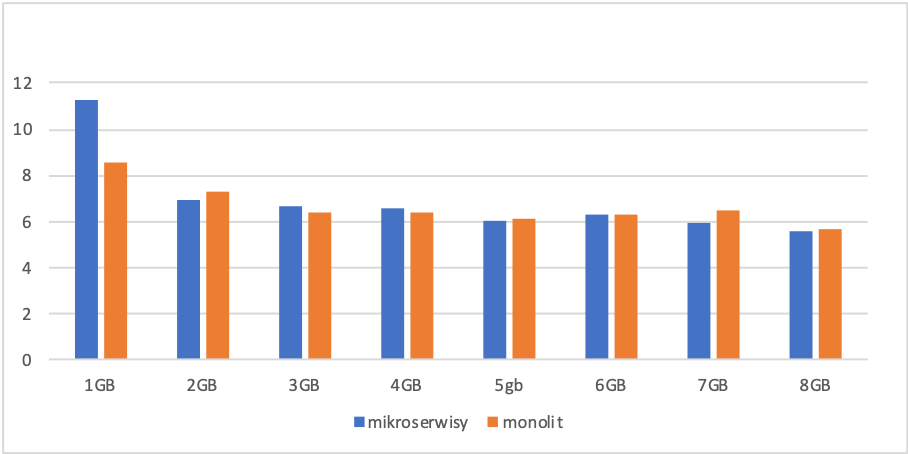
\includegraphics[width=12cm]{Rysunki/Rozdzial7/ramtest.png}
		\caption{Średnie czasy(ms) żądań w zależności od liczby posiadanej pamięci \textit{RAM}.}
		\label{fig:ramtest}
	\end{figure}
\begin{figure}[h!]
	\centering
		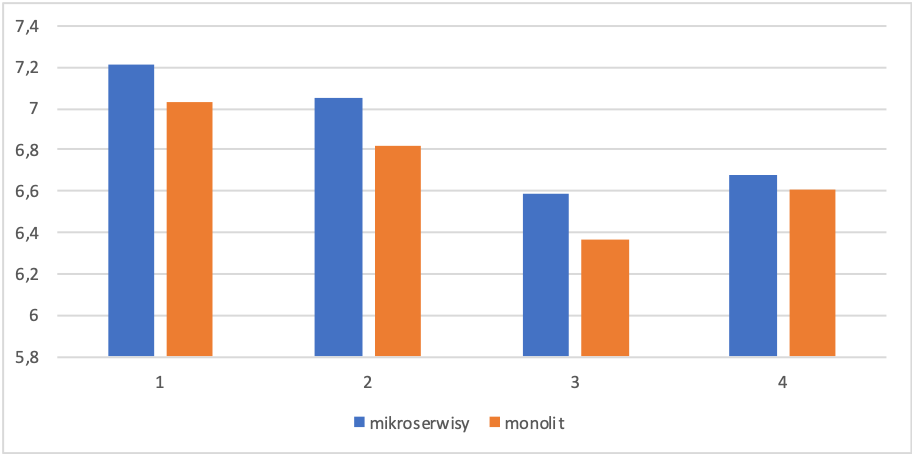
\includegraphics[width=12cm]{Rysunki/Rozdzial7/cputest.png}
		\caption{Średnie czasy żądania(ms) w zależności od liczby rdzeni w procesorze (\textit{CPU}).}
		\label{fig:cputest}
	\end{figure}
Na wykresie \ref{fig:ramtest} widać, że przy niewielkiej ilości pamięci \textit{RAM} ma on wpływ na działanie aplikacji szczególnie, gdy jest go niewiele, wówczas czasy żądań się wydłużają. Prawdopodobnie jest to związane~z tym, że serwisy wymagają minimalnej jego ilości do stabilnego działania, gdy ta zostanie osiągnięta to rola pamięci \textit{RAM} w szybkości obsługiwanych zapytań jest już mniej istotna~i czasy te pozostają na podobnym poziomie. 
Inną zależność można zauważyć~w przypadku liczby rdzeni na wykresie \ref{fig:cputest}, ich ilość nie wypływa na szybkość żądań, dopóki nie będzie ich więcej niż dwa. Każdy użytkownik to asynchroniczne zapytanie. W taki sposób program \textit{Boom} symuluje ruch na serwerze\cite{Ziade:2018}. Prawdopodobnie dwa rdzenie są wykorzystywane przez inne usługi~i zwiększenie ich ilości powoduje, że aplikacja lepiej sobie radzi~z obsługą zapytań, co może tłumaczyć spadek średniej czasów żądań przy trzech rdzeniach.

Następnym przeprowadzonym badaniem jest sprawdzenie skalowalności poziomej dla obu aplikacji, czyli tego jak zachowają się serwisy, gdy zwiększona będzie ilość ich instancji. \textit{Load balancer} zaimplementowany~w każdym~z nich powinien kierować ruchem tak, aby nie obciążać tylko jednego~z kontenerów, co powinno przyczynić się do szybszych czasów żądań\cite{Rodger:2019}.


\begin{figure}[h!]
	\centering
		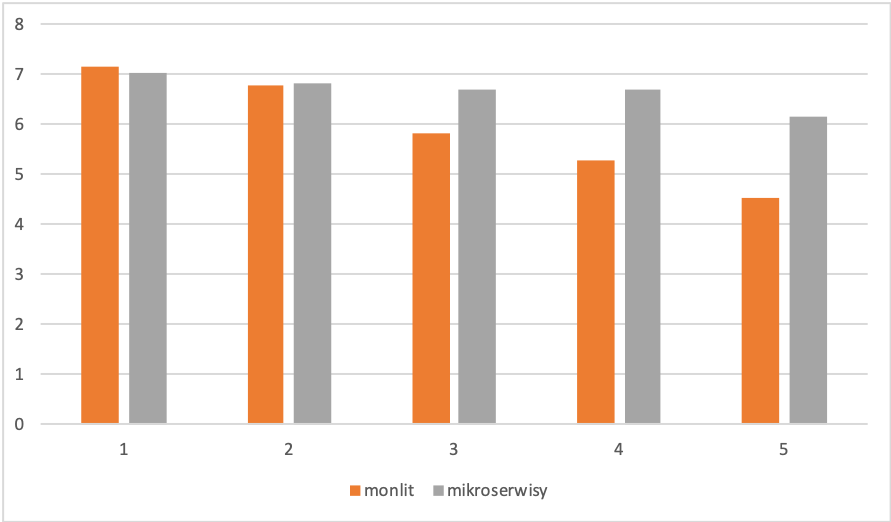
\includegraphics[width=12cm]{Rysunki/Rozdzial7/kontenery.png}
		\caption{Średnie czasy żądania(ms) w zależności od liczby powielonych kontenerów na jeden serwis.}
		\label{fig:kontenery}
	\end{figure}
	
W przypadku	badania skalowalności na wykresie \ref{fig:kontenery} widać tendencję spadkową, która jest zauważalnie większa przy aplikacji monolitycznej. Dla tego serwisu można również dostrzec, że przy liczbie kontenerów \textit{1}, radził on sobie nieznaczenie gorzej od mikroserwisów. Następnie dla dwóch kontenerów oba serwisy miały zbliżone czasy. Dopiero przy kolejnych pomiarach scentralizowana usługa uzyskała przewagę. Posiada ona jeden serwis napisany~w bibliotece \textit{Flask}, co sprawia, że ich skalowanie mniej obciąża maszynę. W aplikacji opartej~o mikrousługi potrzebne było stworzenie wielu instancji dla kilku usług, co~w ostateczności mogło mocniej obciążyć jednostkę, na której testowano serwisy~i zwiększyć czasy żądań aplikacji. 

Przeglądając otrzymane wyniki można zauważyć, że serwis mikrousługowy~w każdym~z porównań wypada gorzej, mimo, że to jego architektura zorientowana jest na łatwą skalowalność\cite{Rodger:2019}, to monolit wykorzystujący hierarchię klas do komunikacji, ma lepszą wydajność. Prawdopodobnie ilość potrzebnych serwisów~w aplikacji mikrousługowej jest niewspółmierna do obsługiwanych danych, rozmiarów projektu~i~w badanych warunkach zastosowane rozwiązania nie przynoszą żadnych dodatkowych korzyści~w polepszeniu wydajności aplikacji, a nawet wpływają na nią negatywnie.

\section{Analiza implementacji projektu}
Wskaźniki wydajności są istotne, ponieważ to one mogą być podstawą do rozważenia przejścia na daną architekturę. Inną decydującą cechą jest łatwość implementacji. To jakie rozwiązania należy zastosować, ich konfiguracja~i wykorzystywane technologie.

Aplikacja monolityczna głównie opiera się~o bibliotekę \textit{Flask} i proste szablony \textit{HTML}, których konfiguracja jest podstawowa. Wszystkie dodatkowe opcje, takie jak formularze są dostarczane przy pomocą zewnętrznego modułu \textit{Flask WTF}, a ich renderowanie odbywa się automatycznie przy pomocy metody \textit{render\_template}.
Do zarządzania sesją użytkownika również wykorzystywano dodatkową bibliotekę, która sprawia, że konfiguracja jest automatyczna, a dodatkowo wprowadza ona możliwość sprawdzenia danych klienta nawet~z szablonów, oferując globalny obiekt \textit{current\_user}. Nie jest potrzebne pobieranie danych~z bazy, a wylogowywanie użytkownika sprowadza się wyłącznie do wykorzystania funkcji \textit{logout\_user()}. 
Struktura projektu monolitycznego jest logiczna, wszystkie elementy aplikacji, które nie współgrają bezpośrednio są od siebie odseparowane, a konfiguracja aplikacji opiera się na przekazaniu niewielkiej ilości zmiennych globalnych~i podłączeniu~z bazą danych. Nie musi on być uruchamiany wewnątrz kontenera, aby komunikować się~z innymi komponentami, a projekt mógłby być bez problemu uruchomiony~i skonfigurowany nie wykorzystując platformy \textit{Docker}.

W przypadku aplikacji opartej na mikrousługach jej decentralizacja sprawia, że każdy~z serwisów jest osobno konfigurowany. Muszą one korzystać~z różnych bazy danych, co tworzy wiele utrudnień takich jak potrzeba powielania plików~z ustawieniami~i wielokrotne instalowania tych samych zależności. Struktura pomniejszych usług przypomina małą aplikację monolityczną, co sprawia, że~w każdej~z nich należy zaimplementować takie same mechanizmy obsługi żądań~i komunikacji~z usługą bazodanową. Zarządzenie sesjami użytkownika opiera się~o zewnętrzny mechanizm, z którym usługi muszą łączyć się przy pomocy protokołu \textit{HTTP} w celu autoryzacji. Baza danych tej usługi musi przechowywać wszystkie stworzone \textit{tokeny} i sprawdzać ich poprawność, co jest rozwiązaniem bardziej skomplikowanym niż zautomatyzowany proces uwierzytelniania~z aplikacji monolitycznej. Dodatkowo należy dbać~o integralność danych, sprawdzać~w każdej~z usług, nawet interfejsie użytkownika, czy żądanie posiada \textit{token}, a następnie przesyłać go dalej~w celu jego odszyfrowania.

Kilka baz danych to też problem~z ich zarządzaniem, potrzebne jest wdrażanie trzech osobnych migracji~i tworzenie tabel. Natomiast po stronie klienta, w przeglądarce internetowej potrzebne było wykorzystanie jej pamięci wewnętrznej (\textit{localStorage}) do przechowywania informacji~o użytkowniku~i wygenerowanych tokenów.

Interfejs użytkownika nie jest zbiorem kilku szablonów~w języku \textit{HTML}, ale osobną aplikacją zbudowaną przy pomocy programu generującego, który tworzy projekt~z wszystkimi strukturami~i konfiguracjami. Do swobodnego korzystania~z wszystkich bibliotek~w nim zawartych~i dowolnego ich konfigurowania, należy poznać wiele modułów frameworka \textit{Nuxt.js}. Są to znaczne ilości dodatkowych warstw abstrakcji~i ustawień~w projekcie.

Poszczególne aplikacje mogą działać osobno, ale tylko razem są możliwe do użytkowania, a do tego potrzebne jest stworzenie wielu plików konfiguracyjnych, niejednokrotnie~z powielonymi informacjami. Kontenery muszą wykorzystywać mechanizmy platformy \textit{Docker} do porozumiewania się, inaczej trzeba by było tworzyć fizyczne struktury sieciowe, a moduł do uwierzytelniania musiałby być widoczny jednie dla pozostałych serwisów wewnątrz prywatnej sieci, aby mógł bezpiecznie pobierać~i przekazywać dane.

Analizując oba podejścia widoczne jest, że aplikacja oparta~o mikroserwisy jest~o wiele trudniejsza do wdrożenia, czas jej stworzenia był dłuższy, wymagała ona skrupulatnego obmyślenia całej architektury, warstw komunikacji pomiędzy poszczególnymi elementami~i ręcznego wdrożenia wielu mechanizmów takich jak serializacja danych, proces uwierzytelniania użytkowników~i struktura zapytań serwera. Do jej szybkiej konfiguracji niezbędna jest platforma \textit{Docker}. Natomiast aplikacja monolityczna wszystkie te mechanizmy ma zaimplementowane~w ramach dodatkowych bibliotek frameworku \textit{Flask}, a sama struktura plików jest przejrzysta~i dobrze zorganizowana na warstwy logiczne, gdzie żadna~z nich się nie powiela.
\chapter{Dyskusja rezultatów~i wnioski końcowe}
\label{roz8}
W ramach pracy udało się przygotować architekturę dla dwóch aplikacji, jednej opartej~o podejście monolityczne, drugiej~o mikrousługi, a następnie je zaimplementować. Szczegółowo przedstawiono wszystkie założenia~i problemy, które mogą się pojawić podczas tworzenia aplikacji, a także środowisko programistyczne potrzebne do ich uruchomienia. Opisano strukturę bazy danych, wykorzystane biblioteki, wymagania funkcyjne~i niefunkcyjne aplikacji. Następnie omówiono proces tworzenia serwisów, zaprezentowano przykłady wykorzystanego kodu, tłumacząc jego działanie~i zwracając uwagę na jego istotne kwestię. Przeprowadzono proces konteneryzacji projektu, tak aby można było go zintegrować~z dowolną platformą oferującą hosting serwisów internetowych. Przygotowano~i przeprowadzono badania mające sprawdzić różnicę pomiędzy wydajnością aplikacji, ich skalowalnością~i to jak te czynniki wypływają na czasy odpowiedzi żądań. Platformy przeanalizowano pod kątem ich implementacji, tego jak trudne były do osiągnięcia zakładane architektury, jakie technologie były wykorzystane. Uzyskane rezultaty pozwalają na ocenę obu podejść. 
\textit{Richard Rodger} w książce \textit{Tao mikrousług. Projektowanie~i wdrażanie}, napisał, że: \begin{quotation}
  Mikrousługi nie są cudownym panaceum, dzięki któremu możesz~z dnia na dzień rozwiązać wszystkie swoje problemy związane~z rozwojem oprogramowania\cite{Rodger:2019}.
\end{quotation}
Wyniki badań jasno przedstawiły, że powyższe stwierdzenie jest prawdą. Mikrousługi posiadają szereg atutów, takich jak to, że ich implementacja nie musi sprowadzać się do jednego projektu, w danym języku, a dzięki uniwersalnemu sposobowi komunikacji pomiędzy komponentami możliwości ich rozwoju jest wiele. Każda~z poszczególnych usług ma swój zakres odpowiedzialności, który jest łatwy do przestrzegania, natomiast trudniejsze do osiągnięcia jest to, aby dane dwie mikrousługi powielały go. Istotne jest to, że każda~z usług to osobny projekt, który nie musi być tworzony przez jeden zespół, tylko kilka równolegle. Co~w zasadzie sprawia, że sama aplikacja posiada więcej możliwości, jeżeli chodzi~o jej skalowanie, można tworzyć instancję dla poszczególnych usług, które są najbardziej obciążone~i im przekazywać najwięcej zasobów, aby działały wydajniej. Niestety przy tak niewielkich aplikacjach jak te stworzone~w ramach niniejszej pracy, rozwiazanie oparte~o mikrousługi okazało się powodować, że podział architektury był zbyt skomplikowany. Stworzenie osobnych serwisów, które musiały się~z sobą porozumiewać~w celu uwierzytelniania tokenów, a także~w warstwie interfejsu użytkownika sprawiło, że liczba interakcji wewnątrz sieci niepotrzebnie wzrosła, dodatkowo ją obciążając. Innym niekorzystnym zjawiskiem było powielanie kodu~i danych, implementowanie tych samych mechanizmów do obsługi bazy danych dla trzech aplikacji, wykorzystywanie identycznych plików konfiguracyjnych. Wnioski~z tych obserwacji potwierdzają przeprowadzone badania, gdzie aplikacja monolityczna~o wiele lepiej radzi sobie~z wydajnością, a nawet skalowalnością. Mimo, że to jedna centralna aplikacja to~i tako możliwe było stworzenie jej kilku instancji, których ruch był obsługiwany przez \textit{load balancer}, dzięki czemu~w tych testach wypadła lepiej od serwisu opartego~o mikrousługi. Nie mniej jednak także ta architektura posiada wady, takie jak potrzeba utrzymywania jednego projektu, opartego~o hierarchię klas, gdzie obsługa ich zakresów~i uprawień spoczywa na programiście. Poszczególne komponenty nie są już tak odizolowane jak~w aplikacji mikrousługowej, co może doprowadzić do zawiłości~i mieszania się odpowiedzialności. To~w rezultacie sprawia, że trudniej jest utrzymać porządek~w kodzie. Gdy jedna mikrousługa będzie wymagała usprawnienia, to wystarczą zmiany wyłącznie~w jej ramach, bez zmian~w całym systemie, co jest niemożliwe~w aplikacji monolitycznej. Także możliwości skalowania serwisu są ograniczone, można uruchomić kilka instancji, ale nie jest to tak elastyczne rozwiazanie jak~w przypadku mikrousług. Analiza wykazała, że wady te nie są istotne przy niewielkich projektach, w przypadku aplikacji monolitycznych~o wiele łatwiej jest rozpocząć projekt, wymaga on mniej konfiguracji. Centralna baza danych jest~o wiele prostsza~w utrzymaniu~i porządkowaniu danych. Architektura centralna jest także, tą przedstawianą~w dokumentacjach projektów\cite{flask} i jej odwzorowanie, a także zaprojektowanie jest~o wiele prostsze. Dodatkowo istniej wiele zewnętrznych modułów pozwalających na znaczne uproszczenie poszczególnych mechanizmów, takich jak uwierzytelnianie, przesyłanie formularzy, czy obsługa danych. 

Przeprowadzone badania wskazują na lepszą wydajność serwisu monolitycznego, ale należy zwrócić uwagę, że stworzona aplikacja jest niewielka, generowane przez nią szablony \textit{HTML} były małej wielkości. Mikrousługi pomimo, że przesyłają jedynie obiekty \textit{JSON}, to muszą je jeszcze serializować, co mogło obciążyć aplikację bez uwidaczniania zalety tego rozwiązania. Dodatkowo usługi uruchomione byłby wewnątrz kontenerów, które mimo tego, że mogą być stosowane~w rozwiązaniach produkcyjnych, to wymagają więcej zasobów. Uruchamianie większej ilości kontenerów~w przypadku aplikacji zdecentralizowanej również mogło wpłynąć na czasy ich odpowiedzi. Innym czynnikiem, który mógł wpłynąć na badania były ograniczenia sprzętowe fizycznej maszyny. Nie była to jednostka przygotowana~z myślą wyłącznie~o rozwiązaniach serwerowych~i posiadła ona ograniczoną liczbę pamięci \textit{RAM}, procesor starszej generacji~i niewielką przestrzeń dyskową. Niemniej jednak przeprowadzone badania miały wyłącznie cel porównawczy, a ich wyniki świadczyć mogą, że zgodnie~z tezą \textit{Richarda Rodgera}, mikrousługi nie wszędzie sprawdzą się jako rozwiazanie najbardziej optymalne\cite{Rodger:2019}.

Ostatecznie można przejść do wniosku, że wybór pomiędzy architekturą monolityczną, a mikrousługami powinien być kierowany głównie ze względu na charakter projektu. Jeżeli ma on być tworzony~w ramach większego zespołu znającego kilka technologii, rozsądne byłoby podzielenie go, tak aby każdy~z nich pracował nad osobną usługą, wówczas przy większych serwisach, możliwe będzie, że wady rozwiązania opartego~o mikrousługi będą mniej istotne. Większa organizacja będzie mogła zainwestować pieniądze~w infrastrukturę sieciową, tak aby odpowiednio przystosować ją do rozwiązań zdecentralizowanych. 

Architektura monolityczna to nadal dobry pomysł na mniejsze aplikacje, gdzie zespół nie składa się~z dużej liczy osób znających kilka technologii. Rozpoczęcie projektu jest wówczas~o wiele prostsze, a wdrożenie takiej aplikacji szybsze. W razie, gdyby urósł on do większych rozmiarów istnieje opcja przepisania go na mniejsze aplikacje~i zmiana architektury na tą opartą~o mikrousługi.

Każdy przypadek aplikacji powinien być indywidualnie przemyślany. Zespół musi być świadomy wszystkich wad~i zalet danych architektur, przewidzieć przyszłe koszty infrastruktury, a także zaplanować czas na niezbędne konfigurację wybranych rozwiązań. Realizacja projektu~w ramach niniejszej pracy pokazała jak istotnym elementem aplikacji internetowych jest ich konfiguracja, odpowiednie zaplanowanie systemu komunikacji między danymi komponentami~i opracowanie architektury tak, aby nie powielała ona niepotrzebnie poszczególnych modułów. W ramach usprawnienia obecnej implementacji projektu mikrousługowego można byłoby inaczej zaplanować odpowiedzialność poszczególnych serwisów, zrezygnować~z osobnego modułu uwierzytelniania~i wielu baz danych. Podzielić cały system jedynie na dwie usługi, jedną odpowiedzialną za przetwarzanie~i przechowywanie wszystkich informacji, drugą za interfejs użytkownika. Byłby to idealny kompromis między architekturą monolityczną~i mikrousługami.


%========================================================================================
% Dodatki
%========================================================================================
\begin{appendix}
	\appendix
	\chapter{Tabele wyników wykorzystanych do stworzenia wykresów}
%=================================================================================================
W ramach przeprowadzonych badań przygotowano następujące tabele, które następnie wykorzystano do stworzenia wykresów opracowanych w głównej części pracy:

\begin{table}[h!]
\centering
\caption{Czasy żądań (ms) dla każdego z adresów w aplikacji monolitycznej.}
\begin{tabular}{|l|r|r|r|}
\hline
\textbf{Adres}  & \textbf{średnia}   & \textbf{najszybszy} & \textbf{najwolniejszy} \\ \hline
/index             & 0,8216 & 0,1702     & 1,0862 \\ \hline
/index - logged    & 1,4356	& 0,1791	 & 1,7834 \\ \hline
/login             & 1,2667	& 0,2167	 & 1,7762 \\ \hline
/users - POST      & 1,2843	& 0,2329	 & 1,6195 \\ \hline
/logout	           & 2,3735	& 0,7693	 & 3,7333 \\ \hline
/tasks - GET       & 0,8025	& 0,0479     & 0,2177 \\ \hline
/tasks - POST      & 1,8744	& 0,2447	 & 2,2621 \\ \hline
/tasks/id.         & 1,7152	& 0,2233	 & 2,1407 \\ \hline
/update-task/id    & 2,0891	& 0,9121	 & 3,6156 \\ \hline
/delete-task/id    & 1,9022	& 0,3753	 & 2,2752 \\ \hline
/404               & 0,5871	& 0,1475	 & 0,8700 \\ \hline
\end{tabular}
\end{table}

\begin{table}[h!]
\centering
\caption{Średnie czasy żądań (\textit{ms}) w zależności od liczby posiadanej pamięci \textit{RAM} (\textit{GB}).}
\begin{tabular}{|l|r|r|r|r|r|r|r|r|}
\hline						
\textbf{Serwis/ \textit{RAM}} & \textbf{1GB}  & \textbf{2GB}	& \textbf{3GB}	& \textbf{4GB}	& \textbf{GB}	& \textbf{6GB}	& \textbf{7GB}	& \textbf{8GB} \\ \hline
mikrousługi  & 11,2469	& 6,8961	& 6,7101	& 6,5419 & 6,0812 & 6,3221	  & 5,991	& 5,5612 \\ \hline
monolit	      & 8,6012	& 7,3012	& 6,4191	& 6,3814 & 6,1328 & 6,3112	  & 6,5312  & 5,7131 \\ \hline
\end{tabular}
\end{table}

\begin{table}[h!]
\centering
\caption{Czasy żądań (ms) dla każdego z adresów w aplikacji opartej o mikrousługi.}
\begin{tabular}{|l|r|r|r|}
\hline
\textbf{Adres}  & \textbf{średnia}   & \textbf{najszybszy} & \textbf{najwolniejszy} \\ \hline
/index              & 0,5957	& 0,2217	& 0,9042 \\ \hline
/index - logged     & 1,1632	& 0,2763	& 2,5775 \\ \hline
/login              & 1,5587	& 0,6577	& 2,9107 \\ \hline
/users - POST       & 2,3541	& 0,8331	& 3,0011 \\ \hline
/users.             & 0,5594   	& 0,1804	& 0,8861 \\ \hline
/logout             & 2,0031	& 0,9011	& 2,8993 \\ \hline
/tasks - GET        & 0,5754	& 0,1902	& 0,8965 \\ \hline
/tasks - POST		& 2,5665	& 0,5664	& 3,2221 \\ \hline
/tasks/id - GET		& 1,1123	& 0,3561	& 2,4412 \\ \hline
/tasks/id  - PUT	    & 4,5511	& 0,7656	& 3,7732 \\ \hline
/tasks/id - DELETE  & 4,8133	& 0,5589	& 3,5581 \\ \hline
/404				& 0,5605	& 0,1984	&0,74620 \\ \hline
\end{tabular}
\end{table}

\begin{table}[h!]
\centering
\caption{Średnie czasy żądań(ms) w zależności od liczby rdzeni w procesorze (\textit{CPU}).}
\begin{tabular}{|l|r|r|r|r|}
\hline
\textbf{Serwis/ \textit{CPU} (rdzenie)}       & \textbf{1}	& \textbf{2}	& \textbf{3}	 & \textbf{4} \\ \hline
mikrousługi & 7,2156	& 7,0517	& 6,5919	& 6,6790 \\ \hline
monolit	     & 7,0357	& 6,8230	& 6,3658	& 6,6058 \\ \hline
\end{tabular}
\end{table}


\begin{table}[h!]
\centering
\caption{Średnie czasy żądań(ms) w zależności od liczby powielonych kontenerów na jeden serwis.}
\begin{tabular}{|l|r|r|r|r|r|r|}
\hline
\textbf{Serwis/ Liczba kontenerów} &	\textbf{1}	    & \textbf{2}	        & \textbf{3}	        & \textbf{4}            & \textbf{5} \\ \hline
mikrousługi	      & 7,0349	& 6,8001	& 6,6881	& 6,6766	    & 6,1601 \\ \hline
monlit	          & 7,1432	& 6,7775	& 5,8308	& 5,2573	    & 4,5396 \\ \hline
\end{tabular}
\end{table}
Badania przeprowadzono na maszynie wyposażonej w procesor \textit{2.7 GHz Intel Core i5} o pamięci RAM \textit{8 GB 1867 MHz DDR3}. Do ich zrobienia wykorzystano narzędzie \textit{Boom} w konfiguracji \textit{100} użytkowników, którzy wysyłali maksymalnie \textit{1000} żądań.
%=================================================================================================
 
\end{appendix}

%========================================================================================
% Literatura
%========================================================================================

\begin{flushleft}
	\bibliography{bibliografia/bibliografia}
\end{flushleft}

\end{document}
%========================================================================================
% Koniec dokumentu
%========================================================================================
